% %!TEX root = ../thesis.tex
% %*******************************************************************************
% %****************************** First Chapter *********************************
% %*******************************************************************************



\chapter{Introduction}  %Title of the First Chapter
\label{chapter1}

\newpage

%\textit{[We might have just found] “The secret of life.”}\\
%\rightline{Francis Crick, 1953}

% %********************************** %First Section  **************************************
\section{Endocrine Pancreas: Morphology and Physiology}  %Section - 1.1
\label{sec:sec1-1endopanc}

The pancreas is a glandular organ originating from the endoderm and located in the abdomen, behind the stomach \textbf{\cite{shih_pancreas_2013}}. It plays a \st{vital organ originating from the endoderm} critical role \st{with a central role} in energy homeostasis\st{. The pancreas exerts its effects} by secreting digestive enzymes and releasing metabolic hormones \textbf{\cite{kimmel_molecular_2010, baron_single-cell_2016}}. The pancreas is the only organ with \st{functions both, as an} exocrine and endocrine \st{gland} functions.  
\\\\
\st{The exocrine} Majority of the pancreatic mass (\textasciitilde 90\%) is comprised of the exocrine tissue, consisting of acinar, centro-acinar and ductal cells \textbf{\cite{pandiri_overview_2014}}. The acinar cells secrete digestive enzymes, which catalyze the breakdown of proteins (peptidases), carbohydrates (amylases), and lipids (lipases). These digestive enzymes are further ferried into the duodenum and the gastrointestinal (GI) tract via the ductal system \textbf{\cite{shih_pancreas_2013, baron_single-cell_2016}}.  In addition to this, the \st{ductal system} pancreatic ducts along with the centro-acinar cells, secrete large volumes of bicarbonate-rich fluid, resulting in the flushing of acinar secretions \textbf{\cite{pandiri_overview_2014, low_pancreatic_2010}}. 
\\\\
The endocrine component, called islets of Langerhans (short islets), comprise 1-2\%, and the interstitium with vasculature, lymphatics, nerves, and fibrous connective stroma make \st{making} up the remainder of the tissue mass \textbf{\cite{pandiri_overview_2014}}. The islets are named after Paul Langerhans, who in 1869, through exhaustive histological studies discovered that the pancreas was a heterogeneous organ comprised of different structures. The islets, embedded within the exocrine tissue and scattered throughout the whole pancreas, consist of several unique cell types, all of which secrete different hormones and peptides for regulating \st{glucose homeostasis}  blood glucose level \textbf{\cite{shih_pancreas_2013, baron_single-cell_2016}} and influencing exocrine function.  The alpha \textbf{(α)} cells release glucagon, the beta \textbf{(β)} cells produce insulin and amylin, the gamma \textbf{(γ)} or PP cells produce pancreatic polypeptide, the delta \textbf{(δ)} cells produce somatostatin and the epsilon \textbf{(ε)} cells produce ghrelin \textbf{\cite{mastracci_endocrine_2012} (Fig. \ref{fig1-1})} . 
\\\\



%\begin{figure}[htbp]
\begin{figure}[ht]
\centering
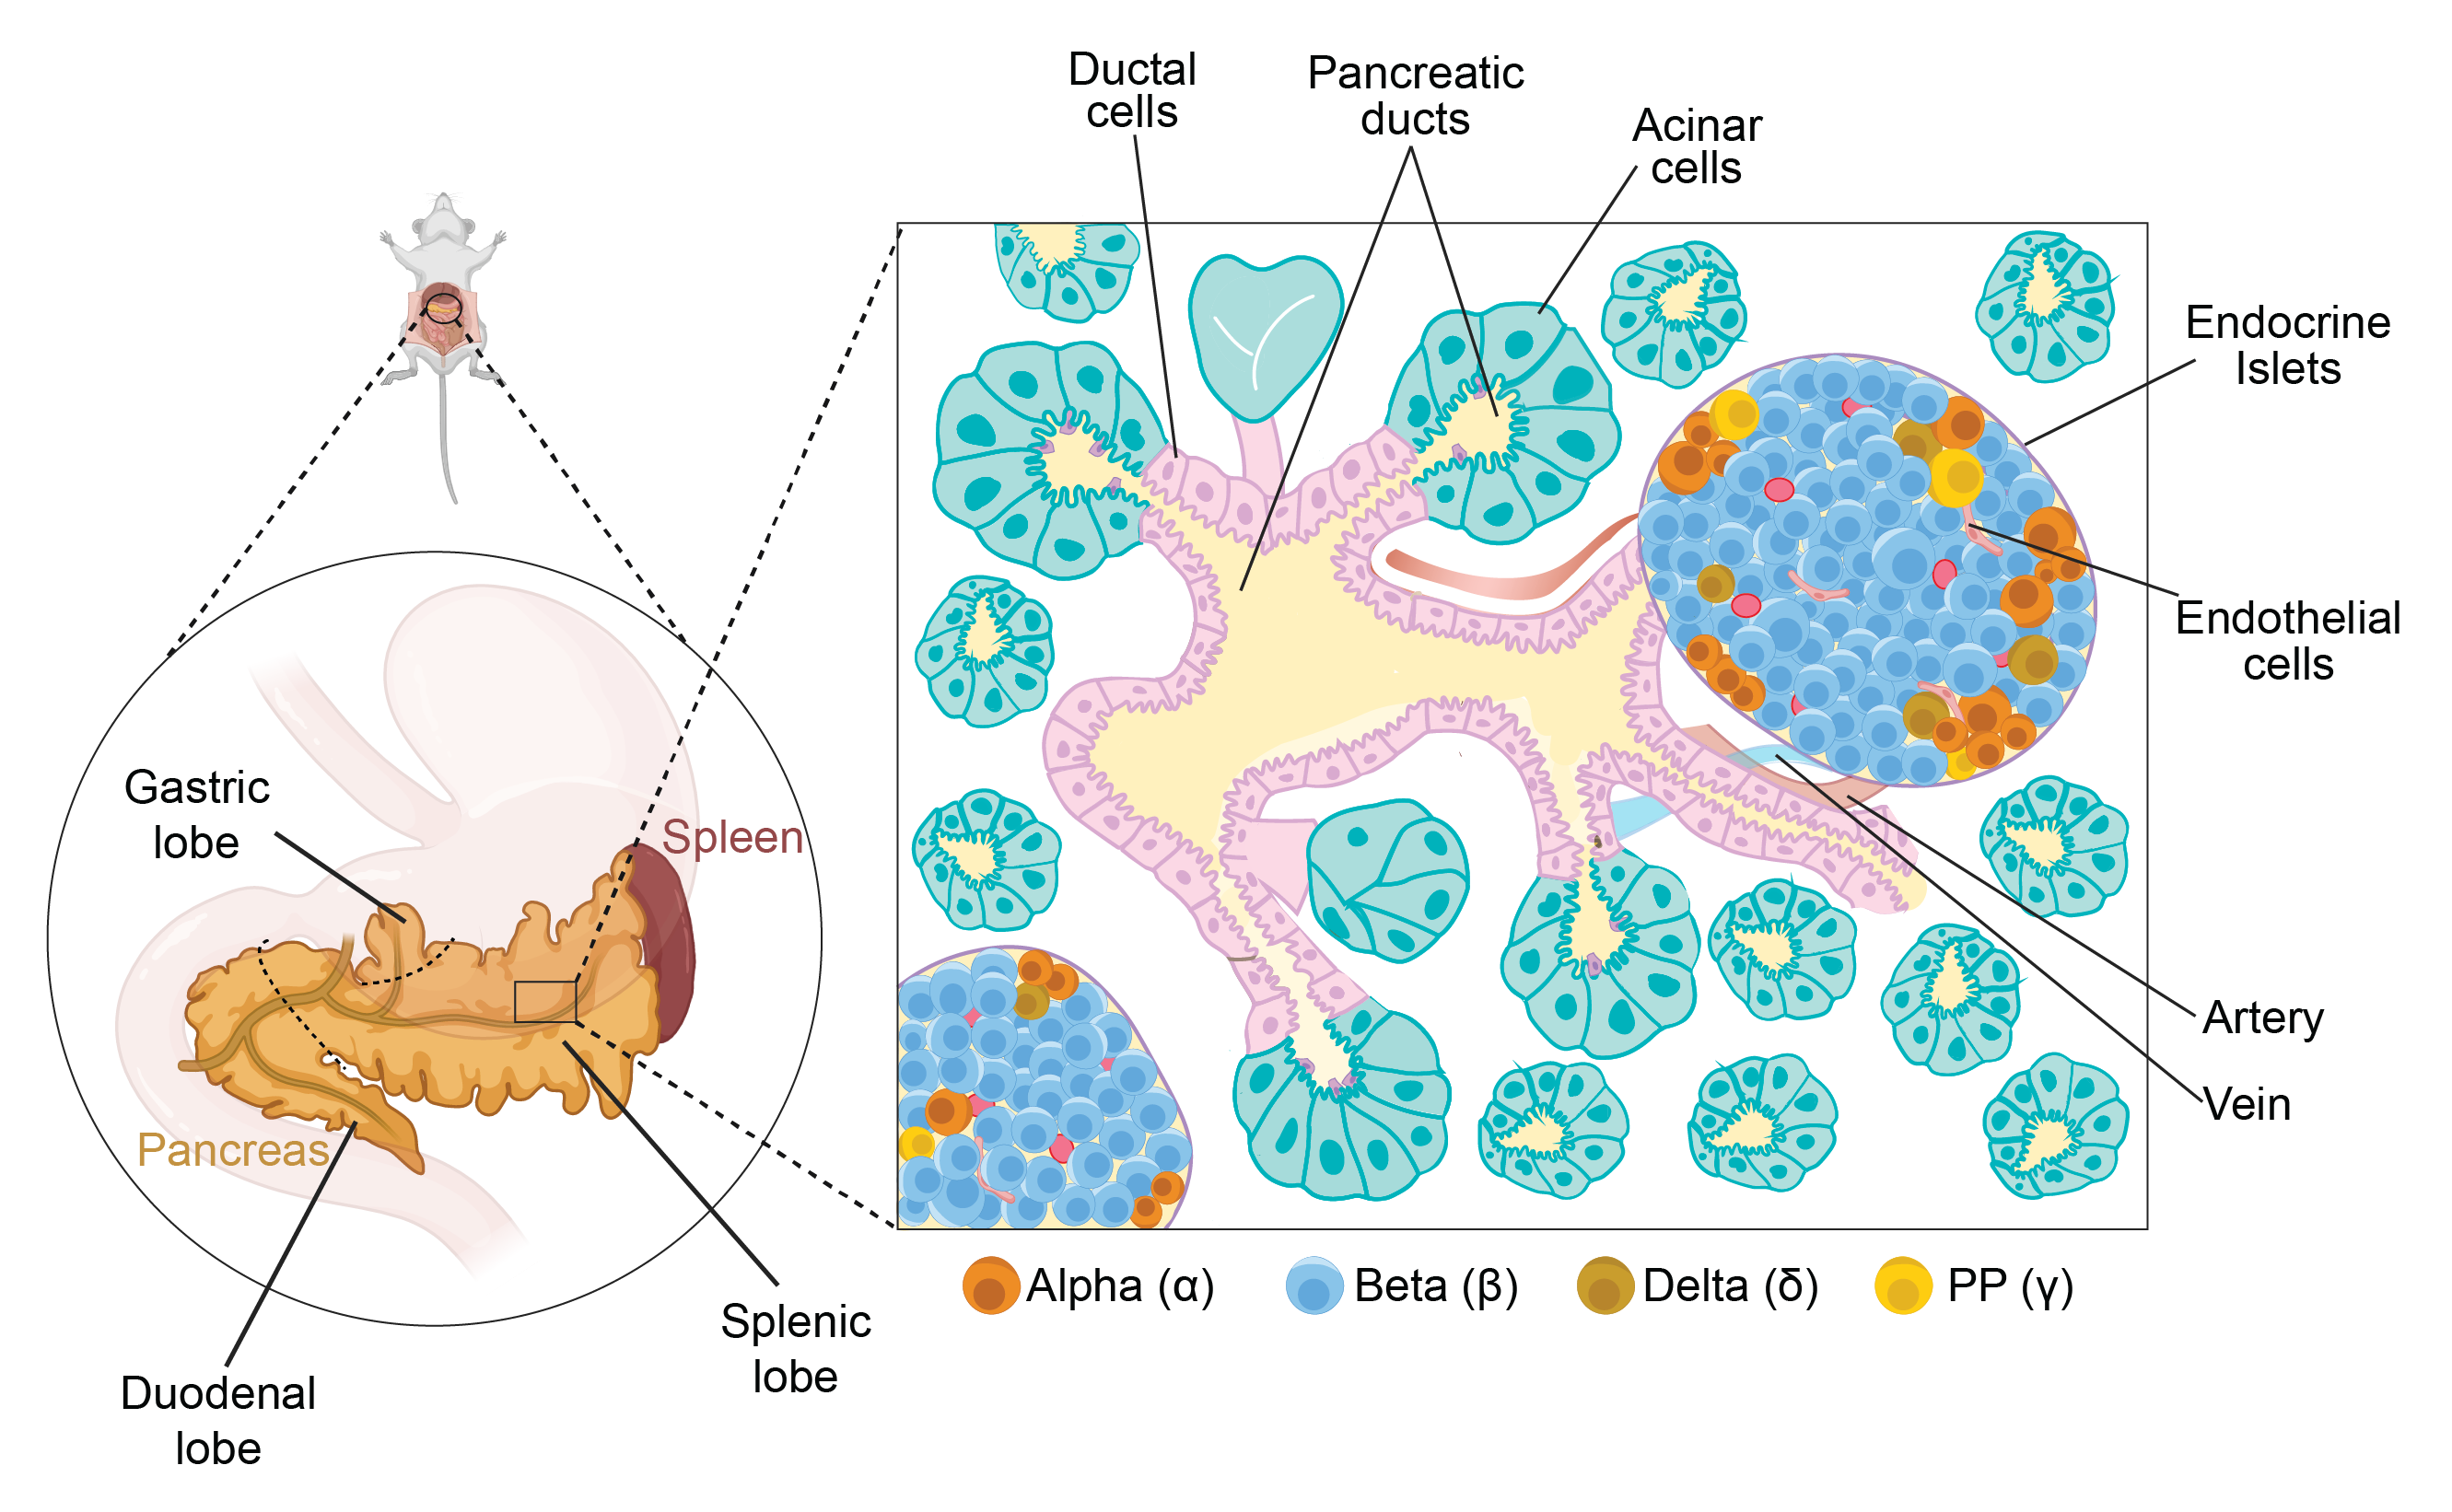
\includegraphics[width=\linewidth]{Chapter1/Fig/F1-1-01.png}
\caption[sec1-1endopanc]{\textbf{Endocrine Pancreas}}
\label{fig1-1}
\end{figure}



The pancreatic tissue in mice is a diffused lobular organ consisting of the duodenal, the splenic, and the gastric lobes. In humans, the pancreas exhibits \st{is} a more compact and well-defined structure, comprising of \st{into three major parts:} the head, the body, and the tail. The pancreas receives a rich vascular supply and the macro-vascular network is conserved in humans and rodents \textbf{\cite{muratore_vascular_2021}}. Although the islets comprise 1-2\% of the pancreas, they receive up to 20\% of the pancreatic blood supply \textbf{\cite{muratore_vascular_2021,jansson_glucose-induced_1986}}. \st{The dense vascularization}This remarkable vascularity of islets is necessary for normal islet function and likely explains how fluctuations in blood glucose are \st{sensed} detected, \st{and lead}leading to rapid and \st{large}substantial changes in the secretion of pancreatic hormones.
\\\\
In rodents such as mice, the islets consist of \textasciitilde75–80\% β-cells, forming a rich “core” and \textasciitilde15–20\% α-cells and the rest is made up by the remaining endocrine cells (δ-cells and PP-cells, <10\% and ε-cells, <1\%), forming the “mantle” of the islet. In contrast, the endocrine cells in the human islets seem to be randomly distributed, and have proportionally fewer β-cells (\textasciitilde55-75\%) and more α-cells (\textasciitilde30-45\%), likely suggesting the major role of glucagon secretion in humans. The variability in cell distribution results in more heterotypic contacts between the endocrine cells in human islets \textbf{\cite{walker_human_2021}}. It has been shown in both mice and humans, that the islet architecture is size-dependent, with smaller islets displaying the core-mantle structure and larger islets with more complex organization \textbf{\cite{dolensek_structural_2015}}. Additional differences in the innervation patterns and presence of smooth muscle cells throughout the vascular network also exist between mouse and human islets \textbf{\cite{rodriguez-diaz_autonomic_2011}}. \st{It is likely that these islet architecture differences between mouse and human}These islet architecture differences between mouse and human likely contribute to physiological differences regarding islet function \textbf{\cite{cabrera_unique_2006}}.
\\\\
To summarize, the pancreatic islets are regarded as a coordinated mini-organ that serves as a remarkable regulator, integrating systemic and local cues to fine-tune blood glucose levels by the synthesis and appropriate secretion of several metabolic hormones by the diverse cell types in the islet microenvironment.

% ********************************** % 1.1.1  **************************************
%\subsection{Principles of (Mendelian) Inheritance} %Section - 1.1.1 
%\label{sec:Mendel}

% ********************************** % 1.1.2 **************************************
% \subsection{Genetic Linkage and the birth of modern genetics} %Section - 1.1.2 
% \label{sec:Morgan}




%%%% Box on genetic terms & origin

%\begin{Comment}
%\hspace{-2.5mm}\textbf{Box 1: Genetic terms \& their origin}\label{box:genetic_terms}
%\small
%\begin{itemize}
%    \item \textbf{Alleles} (originally allelomorphs) were defined by Bateson as the units of inheritance described by Mendel \cite{bateson2013mendel}.
%    \item \textbf{Homozygote} and \textbf{heterozygote} were also used by Bateson to describe individuals carrying the same or different alleles.
%    \item The word \textbf{gene} as a term for the Mendelian factors or units of inheritance was introduced by Danish botanist Johannsen \cite{johannsen1911genotype}. 
%    \item Johannsen also introduced the terms \textbf{phenotype}, as the outward appearance of an individual, and \textbf{genotype}, as their genetic traits. 
%    \item The terms \textbf{polygenetic} (today more often simply polygenic), for traits that are governed by multiple genes, and \textbf{pleiotropic}, for genes that affect multiple, seemingly unrelated, phenotypes also made their first appearance at that time. 
%    \item A \textbf{pedigree}, from the French \textit{pied de grue} (crane's foot), is a diagram that depicts the biological relationships between related individuals.    It is often used to look at the transmission of genetic disorders.
%\end{itemize}
%\vspace{3mm}
%\end{Comment}





% ********************************** % 1.1.3  **************************************
% \subsection{The double helix} %Section - 1.1.3
% \label{sec:double_helix}

% ********************************** % 1.1.4  **************************************
% \subsection{Biometrics} %Section - 1.1.4
% \label{sec:biometrics}

% % %********************************** % 1.1.5  **************************************
% \subsection{Towards quantitative genetics} %Section - 1.1.5
% \label{sec:Fisher}



%\newpage

% % %********************************** % 1.1.6  **************************************
% \subsection{Molecular biology and technological advances}
% \label{sec:genetic_timeline}


% \subsubsection{Cracking the code}
% \label{sec:genetic_code}



% \begin{figure}[htbp]
% \centering
% \includegraphics[width=15cm]{Chapter1/Fig/genetic_timeline_draft.png}
% \caption[Genetic Timeline]{\textbf{150 years of genetics}.\\
% Key scientific discoveries in genetics and corresponding technological advancements.
% A number of scientific discoveries, in combination with key advances in technology and statistical modelling, have led to the identification of thousands of genetic variants which are associated to complex and molecular traits \cite{nhgri2003genetic}.
% Several fundamental contributions have been made, from Mendel's peas to the structure of DNA, to large databases cataloguing genetic variation of hundreds of thousands of individuals.
% Here, I have attempted to highlight the key events that led to today's field of quantitative genetics in the GWAS and post-GWAS era.}
% \label{fig:genetic_timeline}
% \end{figure}

% \subsubsection{Sequencing DNA}
% \label{sec:dna_seq}


% \subsubsection{Understanding the genetic basis of disease}
% \label{sec:disease_genetic}


% \phantomsection
% \label{sec:ld}
% Instead, it was proposed that the combined use of \gls{ld}\footnote{LD: the nonrandom allocation of alleles at nearby variants to individual chromosomes as a result of recent mutation, genetic drift or selection, manifest as correlations between genotypes at closely linked markers \cite{mccarthy2008genome}.} and population- (rather than family-) based studies would be more suitable \cite{risch1996future, jorde2000linkage} - thus practically proposing the design for \glspl{gwas} \cite{risch1996future}.
% However, at the time, implementation of \glspl{gwas} was not possible, for two primary reasons.
% First of all, the technology required to genotype thousands to millions of markers in a single experiment for the larger required sample sizes was not available \cite{risch1996future, visscher2012five}.
% Secondly, the distribution and density of genetic polymorphisms across the genome, and the \gls{ld} between genetic variants across different populations, were unknown.\\

% In some sense, population-based association studies can be viewed as an extension of family-based linkage studies, in which the population studied (derived from common ancestors) acts as an extended pedigree and a much greater number of meiotic recombinations will have occurred between the analysed samples.
% As a consequence, \gls{ld} regions are much smaller than within pedigrees of close relatives, thus requiring a more dense panel of genetic markers to be examined \cite{cordell2005genetic}.

% \subsubsection{The Human Genome Project}
% \phantomsection
% \label{sec:hgp}

% In order to study genomic variation, and therefore its role in disease, it was necessary to generate a reference genome.
% This was the goal of the \gls{hgp}, which aimed at sequencing the entire human genome.
% The \gls{hgp} was 
% % perhaps the first 
% a 
% major breakthrough that dramatically changed the landscape of genetics, and was described by United States President Clinton as “an epic-making triumph of science and reason” \cite{clinton2000remarks} at the announcement of its completion.
% Driven by and a driver of technological breakthroughs in \gls{dna} sequencing and genotyping, the \gls{hgp} was a massive international undertaking and a truly collaborative effort; sequencing and analysis took place across twenty centers in six different countries (USA, UK, France, Germany, Japan, China) and took 13 years to complete, costing approximately \$2.7 billion \cite{lander2011initial}.
% Led in the US by then NIH director Francis Collins and by founder of Celera Genomics \footnote{The company Celera Genomics was formed in May 1998, with the objective of sequencing much of the human genome in three years \cite{venter1998shotgun}.} 
% Craig Venter, and with large contributions from the UK, in particular from the Sanger Institute directed by John Sulston (who had first sequenced the genome of \textit{C. Elegans}), the \gls{hgp} was announced as a joint US-UK statement on June 26th, 2000.
% After a first publication in 2001, the project was truly completed on April 25th, 2003, on the 50$^{th}$ anniversary of the Watson and Crick paper describing the helical structure of \gls{dna}.\\

% The \gls{hgp} provided the first map (obtained from the genomes of a small number of individuals) of the $\sim$3 billion bases in the human genome \cite{lander2001initial, schmutz2004quality, hattori2005finishing}, and revealed that human \gls{dna} consists of surprisingly few exons (1.1\% of the genome), whereas introns cover 24\% of the genome \cite{venter2001sequence, lander2001initial}. 
% Additionally, the number of genes was found to be smaller than expected, with around 30,000 being identified in 2001, and circa 21,000 genes being the latest (still debated) estimate at the time that this thesis is written \cite{pertea2018thousands}. 
% Additional breakthroughs in sequencing technologies have expanded and refined the reference genome, which now captures more than 92\% of the genome and provides a landscape of its genes \cite{lander2011initial}.\\

% With a complete map of the human genome in place, genetic variants could now be identified as those bases discovered in an individual that did not match the (reference) base annotated in the human genome map. 
% Common variants, i.e. variants with \gls{maf}\footnote{The frequency of an
% allele at a genetic locus is the proportion of chromosomes in the study sample that carry that allele \cite{laird2010fundamentals}. 
% For a biallelic variant (a variant for which only two possible alleles are observed in the population), the frequency of the less common (minor) allele is called the minor allele frequency (MAF).} larger than 5\%, were called \glspl{snp}. 
% Previous studies had estimated that approximately 0.1\% (1 base per 1,000) of an individual's genome was a polymorphism \cite{wang1998large, li1991low, cargill1999characterization}. 

% These SNPs were scattered across the genome and it was now time to describe what type of variants they were, where in the genome they were located, and what (if any) effect they had on human phenotypes.

% \subsubsection{The International HapMap Project}

% The International HapMap Project was the first effort of its kind to systematically catalogue genomic variation. 
% Additionally, it aimed to characterise the LD structure of the human genome, which would make GWA studies feasible. 
% The HapMap was officially started in October 2002 as a collaboration between research groups and private companies in Canada, China, Japan, Nigeria, the United Kingdom and the United States with the goal of developing a haplotype map (HapMap) of the human genome \cite{international2003international}.
% By genotyping individuals of African (YRI), European (CEU) and East Asian (JPT, CHB) descent, in Phase I HapMap assembled a publicly available database of common variants (\gls{maf}>5\%) in global samples \cite{international2005haplotype}. 
% The HapMap expanded rapidly. 
% By Phase II (2007), the database contained 2.1 million SNPs from the four original populations \cite{international2007second}.
% Phase III (2010) added genotyping from seven additional populations, for a total of over 3 million SNPs in 11 global ancestry groups\footnote{ASW (African ancestry in Southwest USA); CEU (Utah residents with Northern and Western European ancestry from the CEPH collection); CHB (Han Chinese in Beijing, China); CHD (Chinese in Metropolitan Denver, Colorado); GIH (Gujarati Indians in Houston, Texas); JPT (Japanese in Tokyo, Japan); LWK (Luhya in Webuye, Kenya); MEX (Mexican ancestry in Los Angeles, California); MKK (Maasai in Kinyawa, Kenya); TSI (Tuscans in Italy); YRI (Yoruba in Ibadan, Nigeria).} \cite{international2010integrating}.\\ 

% The growing popularity of genetic association studies in parallel with the expansion of the HapMap effort paved the way for the last needed technological breakthrough: microarrays.
% By knowing the genetic location of thousands of variants, commercial companies were able to develop so-called `SNP chips' \cite{meaburn2006genotyping, oliphant2002beadarray}, which allowed for genotyping at specific locations across the genome.
% In parallel, the data generated by the HapMap project enabled calculation of the LD\footnote{Pearson's correlation coefficient squared, $r^2$, is commonly used} between SNPs within the genome, effectively describing the chance that two SNPs will be inherited together \cite{bush2012genome}.
% This enabled the identification of haplotypes and thus a minimal set of SNPs that capture the majority of the haplotype diversity within a population, called `tag SNPs' \cite{international2003international}. 
% The collective LD information gathered by academics in those years \cite{slatkin2008linkage, pe2006evaluating, otto2002resolving} allowed companies such as Affymetrix and Illumina to develop SNP arrays that contained 
% these tag SNPs, effectively capturing information about common variation across a large percentage of the genome while only directly genotyping a few thousand SNPs.\\

%\newpage

% % %********************************** % 1.1.7  **************************************
% \subsection{Genome-wide association studies}
% \label{sec:gwas}

% The data generated by the International HapMap Project combined with development of appropriate chip-based microarray technology, which enabled simultaneous genotyping of more than one million SNPs, led to the first wave of \glspl{gwas} \cite{visscher2012five}.
% \gls{gwas} are a hypothesis-free\footnote{bar the selection of SNPs on the chip. 
% More recently, shallow DNA-seq has been increasingly used as an alternative, making the approach truly hypothesis-free.} approach to test for statistical association between the genotype frequency of common genetic variants (considered one by one across the genome) and a phenotype of interest \cite{mccarthy2008genome}. 
% The development of GWAS was accompanied by great enthusiasm, and the hope that these studies could better our understanding of the genetic underpinning of human disease, leading to improvement of prognosis and acceleration of drug and diagnostics development. \\

% Initially, \gls{gwas} focused on complex phenotypes with binary outcomes, using a case-control design (i.e. diseased vs healthy).
% Then, for each SNP and binary trait, the association was evaluated using a Cochran–Armitage (trend) test, a $\chi^2$ test or a Fisher's exact test comparing the numbers of cases and controls when stratified by their alleles at the locus of interest. 
% The first successful \gls{gwas} was published in 2002 on myocardial infarction \cite{ozaki2002functional}.
% The same design was then applied in a landmark GWA study conducted in 2005 for age-related macular degeneration (AMD), using 96 cases and 50 healthy controls and testing for associations at $\sim$100,000 SNPs \cite{klein2005complement}. 
% In 2007, the Wellcome Trust Case-Control Consortium (WTCCC) published a study where they performed \gls{gwas} on seven different common diseases, using 2,000 cases for each of bipolar disorder (BD), coronary artery disease (CAD), Crohn's disease (CD), hypertension (HT), rheumatoid arthritis (RA), type I and II diabetes (T1D, T2D) and a common set of 3,000 healthy controls, demonstrating the feasibility of the use of a shared set of controls across several traits \cite{wellcome2007genome}.\\

% A year later, in 2008, the \gls{gwas} Catalog was founded to keep a record of all published \gls{gwas} and identified associations \cite{welter2014nhgri}.
% As of September 2020, when I am writing this thesis, the \gls{gwas} Catalog includes 4,694 publications, describing 197,708 SNP-trait associations \cite{macarthur2017new}.\\

% Over time, quantitative traits have become increasingly popular to use as phenotypes, in addition to binary traits.
% These include continuous traits such as height, weight and blood pressure.
% Furthermore, linear regressions and their derivations have become more popular methods to assess association, due to their flexibility to include covariates \cite{mccarthy2008genome}.
% I describe these models in detail in the next chapter (\textbf{Chapter \ref{chapter2}}). 

%\newpage

% \gls{gwas} results are often visualised using a Manhattan plot \cite{mccarthy2008genome}, where the negative log p value (as a measure of significance) is plotted on the y axis, against the corresponding genomic position (ordered by chromosome and position) on the x axis (\textbf{Fig. \ref{fig:manhattan}}). 
% Peaks on these plots represent loci (multiple variants in \gls{ld}) that display evidence of association with the analysed phenotype. 
% Variants are deemed to be significantly associated with a trait if they exceed an appropriately chosen p value threshold. 

%\begin{figure}[h]
%\centering
%\includegraphics[width=15cm]{Chapter1/Fig/Manhattan_plots_CD_WTCCC_2007.jpg}
%\caption[Manhattan plot]{\textbf{Manhattan plot}.\\
%Manhattan plot for Crohn's disease (CD) from the WTCCC study \cite{wellcome2007genome}.
%On the x axis are plotted the genomic positions of the SNPs tested, one chromosome after %the next.
%On the y axis are the association significance values.  
%Alternating colours are used to distinguish chromosomes (odd numbered chromosomes -and chromosome X- are dark, even numbered chromosomes are light).
%Highlighted in green are statistically significant SNPs (p value < $5 \times 10^{-8}$).}
%\label{fig:manhattan}
%\end{figure}

%\subsubsection{From global traits to molecular traits}

 

% % %********************************** % 1.1.8  **************************************
% \subsection{Expression quantitative trait loci}
% \label{sec:eqtl}

% \subsubsection{Mechanisms of the genetic regulation of gene expression}


% \subsubsection{Mapping eQTL}
% \label{sec:eqtl_map}

 
 
% \subsubsection{\textit{Cis} and \textit{trans} eQTL}



% \begin{figure}[h]
% \centering
% \includegraphics[width=15cm]{Chapter1/Fig/eqtl.png}
% \caption[\textit{Cis} and \textit{trans} eQTL]{\textbf{\textit{Cis} and \textit{trans} eQTL}.\\
% \textit{Cis} eQTL affect the expression of genes directly. 
% \textit{Trans} eQTL, in contrast, affect the expression of typically more distant genes, often by first having a \textit{cis} effect on the expression of intermediate regulatory genes.
% % On the right, the typical representation of eQTL using box plots.
% Figure adapted from \cite{westra2014genome}.
% }
% \label{fig:eqtl}
% \end{figure}



% \subsubsection{From tissue-specific to cell type-specific eQTL}
% \label{sec:eqtl_celltype_specific}



% \subsubsection{Context-specific eQTL}


% \newpage

% \subsubsection{Using eQTL to link genes to disease}
% \phantomsection
% \label{sec:eqtl_gwas}



% \subsubsection{eQTL mapping in iPSC and iPSC-derived cells}



% ***********************************************************************************************************************************************************************************************************************************************************************************************************************************
%\mathbf{\rho}

\newpage

% \vspace*{10px}

% \textit{“It is not birth, marriage, or death, but gastrulation which is truly the most important time in your life.”}\\
% \rightline{Lewis Wolpert, 1986}

% \vspace*{5px}

% ***************************************************************
%************************ %Second Section %****************************************************************
\section{ Islet \( \mathbf{\upbeta} \)-cells}  %Section - 1.2
\label{sec:human_ipscs}  

% ********************************** % 1.2.1  **************************************
\subsection{Pancreas Organogenesis} %Section - 1.2.1 
\label{sec:pancorgano}

Pancreas organogenesis is a \st{highly} conserved process during fetal development and comprises a tightly coordinated and regulated interplay of complex signaling events. During this step-wise program, the pancreas develops from a simple bud-like structure to a \st{final} mature, highly branched organ containing several specialized cell types. In mice, the pancreas specification begins at embryonic day 8.5 \textbf{(e8.5)} with the formation of dorsal and ventral pre-pancreatic regions in the foregut endoderm \textbf{\cite{shih_pancreas_2013, slack_developmental_1995}}. The pancreas development becomes morphologically evident at  \textbf{\textasciitilde e9.5} when the presumptive pancreatic regions in the endoderm undergo thickening and eventually result in the emergence of pancreatic buds \textbf{\cite{shih_pancreas_2013}}. Over the next 2-3 days, the pancreatic buds continue to elongate, accompanied by the stratification of the epithelium and the formation of multiple micro-lumens \textbf{\cite{pan_pancreas_2011}}. At \textbf{\textasciitilde e12.5}, as a result of both due to gut rotation and elongation of the dorsal and ventral stalks, the pancreatic buds (dorsal and ventral) come into contact and fuse into a single organ. \textbf{This early phase of pancreatic development is referred to as the “primary transition”.}

% ********************************** % 1.2.2  **************************************
\subsection{Endocrine Cell Development} %Section - 1.2.2 
\label{sec:endodev}
The vast majority of the endocrine cells arise during the secondary transition from the endocrine progenitors \textbf{\cite{pan_pancreas_2011}}. However, glucagon-containing α-cells can be seen as early as \textbf{e9} in the primordium \textbf{\cite{pictet_ultrastructural_1972,gittes_developmental_2009}}. The fate decision in the bi-potent trunk domain during the secondary transition is determined by graded \textit{Notch} activity. Lower \textit{Notch} activity leads to \textit{Sox9} expression, which is an activator of \textit{Ngn3} \textbf{\cite{shih_pancreas_2013}}, a basic-helix-loop-helix \textbf{(bHLH)} transcription factor \textbf{(TF)} and master regulator of endocrinogenesis \textbf{\cite{gu_direct_2002}}. Cells that do not escape \textit{Notch} signaling express both \textit{Hes1} and \textit{Sox9}, resulting in \textit{Ngn3} repression and eventual contribution to the ductal tree. \st{However, no signals have yet been identified that could account such a segregated expression pattern of Ngn3.} After \textit{Ngn3} expression, endocrine progenitors exit the cell-cycle and delaminate into surrounding stromal tissue \textbf{\cite{shih_pancreas_2013, gouzi_neurogenin3_2011, miyatsuka_neurogenin3_2011}}. These \textit{Ngn3+} cells are uni-potent and as a whole can generate the five different endocrine cell types \textbf{\cite{shih_pancreas_2013,gu_direct_2002,miyatsuka_neurogenin3_2011}}. The timing and strength of \textit{Ngn3} expression determines the efficiency of endocrine cell formation and the cell type: early \textit{Ngn3} expression results in formation of α-cells while delayed expression of \textit{Ngn3}  generates β- and δ-cells followed by γ-cells \textbf{\cite{johansson_temporal_2007}}.
\\\\
Critical TFs such as \textit{Pax4}, \textit{Pdx1} and \textit{Nkx6.1} control the determination of β-cell fate. On the contrary, \textit{Arx} determines α-cell identity. Both \textit{Pax4} and \textit{Arx} are targets of \textit{Ngn3} and are co-expressed, after which they begin to repress each other. In the \textit{Nkx6.1+} β-cell precursors, the switch from the TF \textit{MafB} \st{(v-Maf avian musculoaponeurotic oncogene homolog B)} to \textit{MafA} expression is an important step to activate the complete the β-cell specific program. After birth, immature β-cells undergo stepwise maturation to become fully mature cells.
% ********************************** % 1.2.3  **************************************
\subsection{Postnatal \( \mathbf{\upbeta} \)-cell maturation} %Section - 1.2.3
\label{sec:betamat}
β-cell maturation is continuation of β-cell development and occurs postnatally in mammals (https://link.springer.com/article/10.1007/s00125-022-05672-y). Most of the current understanding of β-cell maturation process is derived from neonatal rodent islets, as similar data from humans is difficult to collect \textbf{\cite{liu_all_2017, salinno_-cell_2019}}. After birth, immature β-cells undergo several steps to become fully mature and functional cells characterized by tightly controlled insulin secretion in response to glucose.
\\\\
The immature β-cells are organized into clusters, forming proto-islets \textbf{\cite{salinno_-cell_2019}}, which eventually undergo structural rearrangements to form the compacted core and mantle architecture \textbf{\cite{sharon_peninsular_2019}}. The developmentally immature β-cells are characterized by a strong proliferative capacity, thereby resulting in a general increase in β-cell mass. The immature β-cells present insulin granules but display “leaky” insulin secretion wherein they have a decreased glucose threshold for stimulated insulin secretion \textbf{\cite{liu_all_2017, blum_functional_2012}} and are less glucose-responsive thereby affecting their ability to regulate insulin secretion in response to fluctuating blood glucose levels. \st{[ref]. <continue from PAI>}
\\\\
Immature β-cells follow a biphasic pattern of maturation \textbf{\cite{salinno_-cell_2019, stolovich-rain_weaning_2015}}.  The first wave starts right after birth and lasts until \textasciitilde 2 weeks, during which β-cells increase the expression of several key TFs and associated machinery necessary to establish adult β-cell identity. Some of the key signature genes include \textit{Pdx1}, \textit{Neurod1}, \textit{Nkx2.2} and \textit{Nkx6.1}, which are expressed by all β-cells at birth \textbf{\cite{salinno_-cell_2019}}. In addition, several other markers have also been identified which mark the early phase of functional maturation of β-cells: increased expression of \textit{Ucn3} \textbf{\cite{salinno_-cell_2019, blum_functional_2012}}, \textit{Syt4} \textbf{\cite{salinno_-cell_2019, huang_synaptotagmin_2018}}, \textit{Fltp} \textbf{\cite{salinno_-cell_2019, bader_identification_2016}}  and dramatic drop in levels of \textit{Npy} \textbf{\cite{salinno_-cell_2019, rodnoi_neuropeptide_2017}}. Among TFs, \textit{MafA} progressively substitutes \textit{MafB} expression and further regulates expression of genes involved in glucose sensing and insulin secretion, thereby characterizing the late phase of postnatal maturation.
\\\\
The second wave of maturation occurs from about the third week of life until the weaning period involving dietary change from high-fat maternal milk to a high-carbohydrate chow diet. During this weaning phase, β-cells begin to exhibit improved glucose-stimulated insulin secretion and glucose-induced replication, although the latter remains to be explained. This phase is characterized by β-cells differentially regulating metabolic pathways, involving a switch from mTORC1 to AMPK-dependent signaling, which defines the mature functional landscape. The dietary change associated with the weaning period also affects the secretion of incretin hormones, which enhance GSIS and modulate β-cell replication.
\\\\
% ********************************** % 1.2.4  **************************************
\subsection{Insulin Biosynthesis} %Section - 1.2.4
\label{sec:insbio}
% ********************************** % 1.2.5  **************************************
\subsection{Glucose-Stimulated Insulin Secretion (GSIS)} %Section - 1.2.5
\label{sec:gsis}

\subsubsection{Triggering \& Amplifying Pathways}
Insulin, secreted by pancreatic β-cells\st{ß-cells} in response to elevated blood glucose levels, is the central anabolic hormone promoting the utilization and storage of metabolic fuel \textbf{\cite{slack_developmental_1995}}. The molecular process wherein hormone release is triggered by a stimulus is called stimulus-secretion coupling.  The release of insulin by a post-prandial increase in glucose concentrations \st{This process} is termed as glucose-stimulated insulin secretion (\textbf{GSIS}), and is the most critical aspect of β-cell\st{ß-cell} identity \textbf{\cite{ashcroft_stimulussecretion_1994}}.  Impaired GSIS is an early marker of β-cell dysfunction and contributes to the pathogenesis of metabolic disorders such as obesity and T2DM \textbf{\cite{jensen_metabolic_2008}}. The canonical pathway for GSIS \st{is made up}consists of two \st{independent yet functionally }distinct components – triggering pathway and amplifying signals \textbf{\cite{henquin_triggering_2000}}. 
\\\\
In the triggering pathway (previously, K\textsubscript{ATP}-dependent pathway), the pancreatic β-cells act as a glucose sensing machinery with the help of glucose transporters (GLUT) embedded in their plasma membranes and respond to changes in blood glucose levels. GLUT2, encoded by \textit{Slc2a2}, is the predominant glucose transporter in rodent β-cells \textbf{\cite{mcculloch_glut2_2011,van_de_bunt_tale_2012}}   and facilitates rapid entry of glucose into the cell, owing to low affinity and high capacity nature. After transmembrane transport (via facilitated diffusion), glucose is metabolized by oxidative glycolysis\st{ via glycolysis, tricarboxylic acid cycle (TCA) and electron transport chain (ETC)}, resulting in the increase of ATP levels and cytosolic ATP / ADP ratio within the cell \textbf{\cite{henquin_triggering_2000}}. β-cells are equipped with ATP-sensitive K\textsuperscript{+} (KATP) channels that undergo closure in an ATP-dependent manner, thereby causing the accumulation of K\textsuperscript{+} ions within the cell and ultimately leading to depolarization of the plasma membrane. This, in turn, results in the opening of voltage-dependent L-type calcium channels (VDCCs), allowing entry of calcium (Ca\textsuperscript{2+}) ions into the cell down the electrochemical gradient by facilitated diffusion. In addition, Ca\textsuperscript{2+} released from intracellular stores also contribute to the rise of cytosolic Ca2+ concentration \textbf{\cite{yang_ionic_2014}}. The increase in intracellular Ca\textsuperscript{2+}, which is the indispensable signal, triggers exocytosis, wherein the insulin-containing secretory granules fuse with the plasma membrane and release insulin into the extracellular space.
\\\\
<SNARE COMPLEX FORMATION>
\\\\
While the triggering signal is sufficient to enact insulin secretion, it is poorly effective \textbf{\cite{henquin_pathways_2004}}. The metabolism of glucose generates additional signals that serve to fine-tune the action of increase in intracellular Ca\textsuperscript{2+} concentrations. This mechanism was shown to work independent of the K\textsubscript{ATP} channels \textbf{\cite{sato_dual_1992,gembal_evidence_1992}}, and was therefore termed as \textbf{K\textsubscript{ATP}-independent pathway}. It is now referred to as the \textit{`metabolic amplifying pathway'} \textbf{\cite{henquin_triggering_2000,henquin_pathways_2004,henquin_regulation_2009}}.  This pathway depends on the initial triggering signal of Ca\textsuperscript{2+} influx and increases the `release compentency' of insulin granules thereby augmenting insulin secretion in a glucose-concentration-dependent manner \textbf{\cite{henquin_triggering_2000,kalwat_mechanisms_2017}}. In addition to glucose, the amplifying pathway can optimize the secretory response to non-glucose stimuli as well \textbf{\cite{henquin_triggering_2000,kalwat_mechanisms_2017,zhao_-hydrolase_2015,tengholm_camp_2017,han_glutamate_2021}}. This amplifying pathway can also be observed in models of K\textsubscript{ATP} channel knockouts which result in constant depolarization of the β-cell \textbf{\cite{nenquin_both_2004,miki_defective_1998,ravier_glucose_2009}}. The exact mechanisms behind the amplifying pathway remain to be elucidated and several amplifying factors such as proteins, metabolites and associated pathways have been proposed \textbf{\cite{kalwat_mechanisms_2017}}.
\\\\
GSIS follows a characteristic `biphasic' pattern – a peak-shaped first phase followed by a coordinated, pulsed second phase \textbf{\cite{grodsky_threshold_1972,ashcroft_diabetes_2012,komatsu_glucosestimulated_2013}}. Researchers have proposed that the biphasic nature reflects the existence of distinct pools of secretory granules within the β-cells, and has also been confirmed by a FRET-based study \textbf{\cite{ashcroft_diabetes_2012,takahashi_snare_2010}}. The rapid but transient first phase last $\sim$5-20 minutes after glucose stimulus, during which pre-docked (by tetrameric complex of proteins) insulin-containing secretory granules near the Ca\textsuperscript{2+} channels, called `readily releasable pool' \textbf{(RRP)} undergo exocytosis, thereby giving a short, boosted secretion curve. The triggering pathway is mainly responsible for this first phase of GSIS \textbf{\cite{kalwat_mechanisms_2017,campbell_mechanisms_2021}} and causes the release of about 1\% of  the RRP \textbf{\cite{campbell_mechanisms_2021}}. In contrast, the second phase exhibits a sustained secretion at a lower rate as new granules from the cell-internal `reserve pool' \textbf{(RP)} replenish the RRP by physical translocating to the plasma membrane before exocytosis. Therefore, Komatsu et. al. proposed viewing the biphasic insulin release as `fusion and replacement' \textbf{\cite{komatsu_glucosestimulated_2013}}. The metabolic amplifying pathway associates with this `second phase' of GSIS \textbf{\cite{kalwat_mechanisms_2017,campbell_mechanisms_2021}} and allows for insulin secretion to continue at a lower but sustained rate for several hours after a meal and accounts for $\sim$60-70\% of the insulin secreted \textbf{\cite{henquin_regulation_2009}}. There is sufficient evidence to demonstrate that amplification is involved during both phases of insulin secretion \textbf{\cite{mourad_metabolic_2010,mourad_metabolic_2011}}.
% ********************************** % 1.2.6  **************************************
\subsection{Regulation of GSIS} %Section - 1.2.6
\label{sec:reggsis}
Besides glucose, β-cells also respond to other nutrients such as amino acids and fatty acids, leading to fuel-induced insulin secretion. In addition, other hormones and neurotransmitters can also modulate insulin secretion by β-cells.\st{The following section discusses a few of these of regulators of insulin secretion:}

\subsubsection{Gut Hormones}
The gut hormones, also known as incretins, are secreted by specialized enteroendocrine cells in the bowel and play crucial roles in regulating glucose homeostasis and other metabolic functions. The incretins exhibit “incretin effect” to stimulate insulin secretion and are responsible for ~ 50 -70\% of the insulin response to glucose. The two main incretin hormones, which are insulinotropic, are:

\begin{enumerate}
    \item\textbf{Glucagon-like peptide 1 (GLP-1)}\\
    GLP-1 affects insulin secretion in a glucose-dependent manner and regulates factors involved in KATP-dependent insulin secretion. GLP-1 binds to GLP-1R and depolarizes the membrane potential by blocking the K-ATP channels, which is a crucial step in the insulin secretion pathway. Further, GLP-1 potentiates the opening of VDCCs by altering the permeability of these channels thereby allowing for more Ca2+ influx and greater insulin secretion \textbf{\cite{meloni_glp-1_2013}}. However, in absence of glucose, GLP-1 has little to no effect on insulin secretion. Besides, GLP-1 has also been shown to modulate β-cell metabolism upon chronic exposure \textbf{\cite{carlessi_glp-1_2017}} and induce β-cell mass expansion by promoting proliferation and inhibiting apoptosis pathways \textbf{\cite{macdonald_multiple_2002}}. 
    \item\textbf{Glucose-dependent insulinotropic polypeptide (GIP)}\\GIP exerts its insulinotropic effects in a similar fashion to GLP-1 and binds to its specific receptor GIPR on β-cells. GIP seems to be a physiological bi-functional blood glucose stabilizer. GIP potentiates insulin secretion in a glucose-dependent manner whereas it enhances postprandial glucagon response \textbf{\cite{seino_gip_2010, christensen_glucose-dependent_2011}}. Furthermore, GIP also facilitates fat deposition in adipose tissues, and promotes bone formation \textbf{\cite{seino_gip_2010}}. In type-2 diabetic individuals, GIP has impaired effect on insulin secretion due to the downregulation of GIPR \textbf{\cite{irwin_therapeutic_2009}}.

\end{enumerate}

\subsubsection{Amino Acids}
Amino acids exert influence on insulin secretion via their mitochondrial metabolism in β-cells to generate metabolic coupling factors. One such factor, ATP, generated via the oxidation of amino acids, suppresses K-ATP channels and activates VDCCs, leading to the exocytosis of insulin granules. The amino acid, L-arginine is considered a powerful secretagogue as well as an essential synergistic compound for nutrient-dependent insulin secretion \textbf{\cite{newsholme_nutritional_2012}}. Certain amino acids also play a crucial role in nutrient-sensing signaling \textbf{\cite{newsholme_nutritional_2012}} and may influence gene expression affecting insulin secretion \textbf{\cite{newsholme_amino_2006}}. In addition, four amino acids (leucine, isoleucine, alanine and arginine) have also been found to be particularly important in stimulating β-cell electrical activity thereby affecting insulin secretion \textbf{\cite{newsholme_amino_2006}}. 

\subsubsection{Fatty Acids}
Fatty acids (FA) can have varied effects on GSIS. Non-esterified long-chain fatty acids potentiate GSIS by strongly amplifying the effect of glucose as opposed to direct triggering of insulin release. This likely suggests an autocrine effect wherein FA’s secreted by β-cells in response to glucose can signal through their receptors and affect GSIS \textbf{\cite{poitout_fatty_2018}}. In low glucose conditions, long-chain FA's can acutely induce insulin secretion via mitochondria-dependent as well as independent mechanisms \textbf{\cite{cen_fatty_2016}}. However, long term exposure to high levels of FA’s can result in lipotoxicity and further impair or inhibit GSIS \textbf{\cite{jezek_fatty_2018}}. Chronic levels of FA’s can decrease insulin biosynthesis and β-cell glucose sensitivity \textbf{\cite{chueire_effect_2020}}. 
\\\\
Apart from the above factors, insulin secretion can also be regulated by other hormones \textbf{\cite{cheng_follicle-stimulating_2023}}, neural inputs via the autonomic \textbf{\cite{thorens_brain_2011, komatsu_glucosestimulated_2013}} and central nervous systems \textbf{\cite{ruud_neuronal_2017}} and neurotransmitters \textbf{\cite{rodriguez-diaz_neurotransmitters_2014}}, reflecting a complex interplay between the various body systems in maintaining glucose homeostasis. 






% ********************************** % 1.2.7  **************************************
\subsection{Insulin Action and Clearance} %Section - 1.2.7
\label{sec:insact}
Insulin exerts its known physiological effects by binding to the insulin receptor (InsR) on the surface of target cells. The InsR assembles as a tetramer, consisting of two extracellular alpha subunit, which binds insulin and a two membrane-spanning beta subunit, with a tyrosine-kinase domain each. The activation of this kinase results in a metabolic signaling cascade downstream, eventually leading to the uptake of glucose, lipids and amino acids into the cells. The two principal pathways resulting from this interaction include the phosphoinositide 3-kinase (PI3K)/Akt pathway and the Ras/mitogen-activated protein kinase (MAPK) pathway. The PI3K/Akt pathway is critical for linking insulin receptor substrate (IRS) proteins to the metabolic actions of insulin whereas the Ras/MAPK pathway is primarily associated with the growth and mitogenic effects of insulin \textbf{\cite{de_meyts_insulin_2000}}. The binding of insulin to InsR in the target tissues stimulates the translocation of glucose transporter 4 (GLUT4) storage vesicles from intracellular pools to the cell surface, thereby increasing the rate of glucose uptake \textbf{\cite{shepherd_glucose_1999,saltiel_insulin_2001,leto_regulation_2012}}. In the absence of insulin, only ~5\% of GLUT4 pool can be found on the plasma membrane \textbf{\cite{leto_regulation_2012}}.\\\\
The principal target tissues for insulin action include the liver, skeletal muscles and white adipose tissue (WAT), although InsR have been found in several other tissues \textbf{\cite{spencer_identification_2018}}.

\subsubsection{Liver}
The liver is exposed to higher insulin concentrations as insulin from pancreas is secreted into portal vein \textbf{\cite{petersen_mechanisms_2018}}. Insulin, along with glucose, regulates hepatic glycogen metabolism and promotes net glycogen synthesis \textbf{\cite{petersen_mechanisms_2018,rossetti_relative_1990,roden_roles_1996}}. Insulin suppresses glycogenolysis and also transcriptionally represses gluconeogenic genes thereby further reducing the hepatic glucose output \textbf{\cite{petersen_mechanisms_2018,claus_regulation_1976,cherrington_direct_1998,edgerton_insulins_2006}}. The hepatic insulin signaling cascade upregulates several genes involved in \textit{de novo} lipogenesis thereby promoting lipid storage in hepatocytes and reduced export of very-low-density lipoprotein (VLDL) \textbf{\cite{petersen_mechanisms_2018,leavens_insulin_2011}} and reducing the availability of FA’s for oxidation by other tissues \textbf{\cite{petersen_mechanisms_2018,dimitriadis_insulin_2011}}. Insulin also mediates protein synthesis in hepatocytes via the mTOR network \textbf{\cite{petersen_mechanisms_2018,ROS}}.

\subsubsection{Skeletal Muscles}
Muscle insulin action accounts for ~75-90\% of the systemic glucose uptake \st{and its subsequent conversion to glycogen via glycogen synthase (GS)}, thereby playing a crucial role in the regulation of whole body energy homeostasis \textbf{\cite{leto_regulation_2012,petersen_mechanisms_2018}}. The surge in glucose uptake \st{leads to an increased concentration of glucose-6-phosphate (G6P), an allosteric activator of GS. Insulin also dephosphorylates and activates GS, which is further sensitized by G6P}promotes glycogen synthesis via gylcogen synthase (GS) \textbf{\cite{sylow_many_2021}}. Similar to glucose uptake via GLUT4, insulin stimulates translocation of several long-chain fatty acid transporters (CD36, FATP1/4) to cell membrane for the uptake of hydrophobic fatty acids and their subsequent metabolic processing and storage \textbf{\cite{sylow_many_2021,luiken_insulin_2002,wu_fatp1_2006,abumrad_membrane_1999}}. Insulin also stimulates amino acid uptake via amino acid transporters LAT1 and SNAT2 \textbf{\cite{sylow_many_2021,drummond_increase_2010}}, promotes subsequent protein synthesis, and curbs skeletal muscle protein breakdown \textbf{\cite{dimitriadis_insulin_2011,sylow_many_2021}}.

\subsubsection{White Adipose Tissues (WAT)}
Insulin stimulates glucose transport in adipocytes, although this accounts for only a small portion of the systemic glucose uptake \textbf{\cite{leto_regulation_2012}}. Insulin is a potent anti-lipolytic hormone and controls the levels of non-esterified fatty acids (NEFA) in plasma by suppression of lipolysis, which is critical for the maintenance of euglycemia \textbf{\cite{dimitriadis_insulin_2011}}. It has been proposed that insulin plays a part in the esterification of fatty acids in adipocytes, which is the predominant lipogenic pathway \textbf{\cite{lewis_disordered_2002}}. Insulin also increases the uptake of FFAs from blood thereby promoting triglyceride esterification and storage \textbf{\cite{czech_insulin_2013}}.\\\\ 

\clearpage

The above actions of insulin on the principal target tissues can be together termed as `direct effects’. \st{These direct effects along with a strong emphasis on downstream signal transduction events are reviewed herehave been the subject of several reviews 73}. In addition to these, insulin is also known to exert important indirect effects, which are less well understood due to the inherent difficulty in modeling these in cell cultures. Islet β-cells express all isoforms of InsR and the downstream signaling components thereby making it a possibility that insulin itself can trigger the insulin-signaling pathway in β-cells and serve an autocrine role. However, whether it serves a stimulatory or inhibitory role and the physiological relevance of this action is still a subject of ongoing research \textbf{\cite{rhodes_direct_2013,rachdaoui_insulin_2020}}.\\\\
Insulin clearance is a crucial process in maintaining the homeostatic level of insulin required to reach the target tissues. The liver is plays a significant role in the clearance of the endogenously secreted hormone, accounting for up to 80\% of insulin degradation, during the first passage through the tissue \textbf{\cite{najjar_hepatic_2019,zaharia_reduced_2023}}. Thus, the liver regulates the flow of insulin into the systemic circulation and insulin action, thereby acting as a gatekeeper \textbf{\cite{cherrington_direct_1998}}. After the first passage, the insulin that is not degraded exits through the hepatic vein and reaches the heart, wherein it is pumped into arterial circulation and delivered to target tissues \textbf{\cite{tokarz_cell_2018}}. The circulating insulin is also subject to peripheral clearance by kidneys (via the glomerulus and proximal tubule) and other target tissues to a limited extent \textbf{\cite{najjar_hepatic_2019,polidori_hepatic_2016}}. After circulation, insulin returns to the liver and undergoes a second passage of clearance. The primary protease responsible for degrading insulin in tissues is known as insulin-degrading enzyme (IDE), and is ubiquitously expressed in tissues and has multiple cellular functions \textbf{\cite{duckworth_insulin_1998}}.  


\clearpage

% %********************************** % 1.2.1  **************************************
% \newpage

% \subsection{From homunculi to developmental biology}
% \label{sec:history_developmental_biology}



% \begin{wrapfigure}{r}{0.6\textwidth}
% \includegraphics[width=9.5cm]{Chapter1/Fig/Early_theories_development.png}
% \caption[Early theories of development]{\textbf{Early theories of development}.\\
% Illustration of the two leading theories on human embryology before the 19$^{th}$ century.
% Left, Illustration of Preformation: 
% A tiny person (homunculus) growing inside a sperm, as drawn by Nicolaas Hartsoeker in 1695.
% Right, Epigenesis: study of foetus deveopment by Leonardo Da Vinci, c. 1510.}
% \label{fig:early_embryology}
% \end{wrapfigure}




%\newpage

% \subsection{}}
% \label{sec:human_embryogenesis}




% \begin{figure}[h]
% \centering
% \includegraphics[width=14.5cm]{Chapter1/Fig/embryogenesis_til_gastrulation.png}
% \caption[Human Embryogenesis]{\textbf{Human Embryogenesis}.\\
% Early stages of human embryogenesis.
% (a) From zygote to morula: stages of clevage.
% (b) The blastocyst.
% Cells divide and form an outer layer, the trophoblasts.
% Inner cells also called embryoblasts get compacted and move to a side forming the inner cell mass (ICM), leaving a fluid filled cavity called the blastocoel.
% (c) The formation of the bilaminar disk.
% The ICM splits into the epiblast and hypoblast which distribute along the surface and result into two more cavities, the amniotic cavity and the primitive yolk sac, respectively.
% (d) Gastrulation: from bilaminar to trilaminar disk.
% The primitive streak forms and cells start to migrate moving down in between the epiblast and the hypoblast.
% The endoderm, mesoderm and ectoderm form and are called the trilaminar disk.}
% \label{fig:embryogenesis}
% \end{figure}

 

% \subsection{Human Stem Cells}
% \label{sec:escs} 


% \begin{figure}[htbp]
% \centering
% \includegraphics[width=16cm]{Chapter1/Fig/stem_cell_potency.png}
% \caption[Stem Cells]{\textbf{The potency tree of stem cells}.\\
% The spectrum of potency along human development: from the totipotent zygote to terminally differentiated cells.}
% \label{fig:stem_cells}
% \end{figure}

% \subsubsection{Embryonic stem cells}
% \label{sec:esc_induction}




% %********************************** % 1.2.3  **************************************
% \subsection{Nuclear cloning of somatic cells}
% \label{sec:cloning} 


% %********************************** % 1.2.1  **************************************
% \subsection{Induced pluripotent stem cells}
% \label{sec:ipsc}
   

%\begin{figure}[h]
%\centering
%\includegraphics[width=15cm]{Chapter1/Fig%/ipsc_timeline.png}
%\caption[iPSCs timeline]{\textbf{Historical timeline of key events leading to the development of iPS cells}.\\
%Key events including somatic cloning and isolation of ES cells that eventually led Shinya Yamanaka and colleagues to generate iPSCs in 2006 and Yamanaka to win the 2012 Nobel Prize for Physiology and Medicine alongside Sir John Gurdon.}
%\label{fig:ipsc_timeline}
%\end{figure}

% \newpage

% \subsubsection{Inducing pluripotency}

% \subsubsection{Challenges in the use of iPSCs}
% \subsubsection{Reprogramming factors}
% \subsubsection{Mechanisms of iPSC induction}



%\begin{figure}[htbp]
%\centering
%\includegraphics[width=14cm]{Chapter1/Fig/ipscs.png}
%\caption[iPS cells]{\textbf{iPS cells - derivation and applications}.\\
%The generation of iPSCs starts with a biopsy from, for example, the skin of an adult donor.
%Adult cells, in the example fibroblasts, are then isolated and pluripotency is induced through four reprogramming factors, for example the Yamanaka factors: Oct4, Sox2, Klf4 and c-Myc (OSKM).
%The factors can be delivered using a number of systems, see \textbf{page \pageref{sec:ipsc_delivery}}.
%The resulting induced pluripotent stem cells (iPSCs) are self-renewing and are virtually indistinguishable from ESCs.
%They can be subsequently differentiated towards other cell types, including disease relevant cell types, for example dopaminergic neurons for Parkinson's disease, or pancreatic beta cells for diabetes.
%In the future, iPSC-derived cells might be used for cell therapy, i.e. they could be transplanted into the patient, with no risk of allogenic rejection.
%In the meantime, iPSCs and iPSC-derived differentiations can be used to model development and disease, and to do compound screening and drug testing.
%Figure created with BioRender.com.}
%%\label{fig:ipsc}
%\end{figure}


% \subsubsection{Delivery methods}
% \label{sec:ipsc_delivery}




% \subsubsection{Somatic cell of origin}
% \label{sec:ipsc_somatic_cell}



% \subsubsection{Characterising iPSCs}
% \label{sec:ipsc_characterise}



% \subsubsection{Heterogeneity of iPSCs and between cell line variation}


% \subsection{Applications of human iPSCs in genetics}
% \label{sec:ips_genetics}





% \subsubsection{HipSci and other human iPSC consortia}
% \label{sec:HipSci}


% \subsubsection{eQTL mapping using iPSCs and iPSC-derived cells}


% \newpage

% %********************************** %Third Section  **************************************
\section{Diabetes Mellitus}

Diabetes Mellitus (DM), commonly referred to as diabetes, is a group of complex metabolic disorders that has reached pandemic proportions, and poses a significant global health challenge. \st{As of 2019, approximately 463 million adults aged 20-79 were diabetic and this number is projected to rise to ~700-800 million by 2045.} The International Diabetes Federation (IDF) reported that 10.5\% of the adult population (20-79 years) had diabetes in 2021, and projected that this proportion would increase to 13.7\% by 2045 (\textbf{Fig. \ref{fig:idf}}) \textbf{\cite{home_idf_nodate}}. In Germany, an estimated 7\% of the adult population was diabetic in the year 2021 \textbf{\cite{noauthor_germany_nodate}}. Diabetes is associated with several long-term complications such as kidney failure, cardiovascular diseases and is a major risk factor for blindness, lower limb amputation, \st{stroke} and stroke and nerve damage \textbf{\cite{ashcroft_diabetes_2012,emerging_risk_factors_collaboration_diabetes_2010,leon_diabetes_2015}}. 

\begin{figure}[H]
\centering
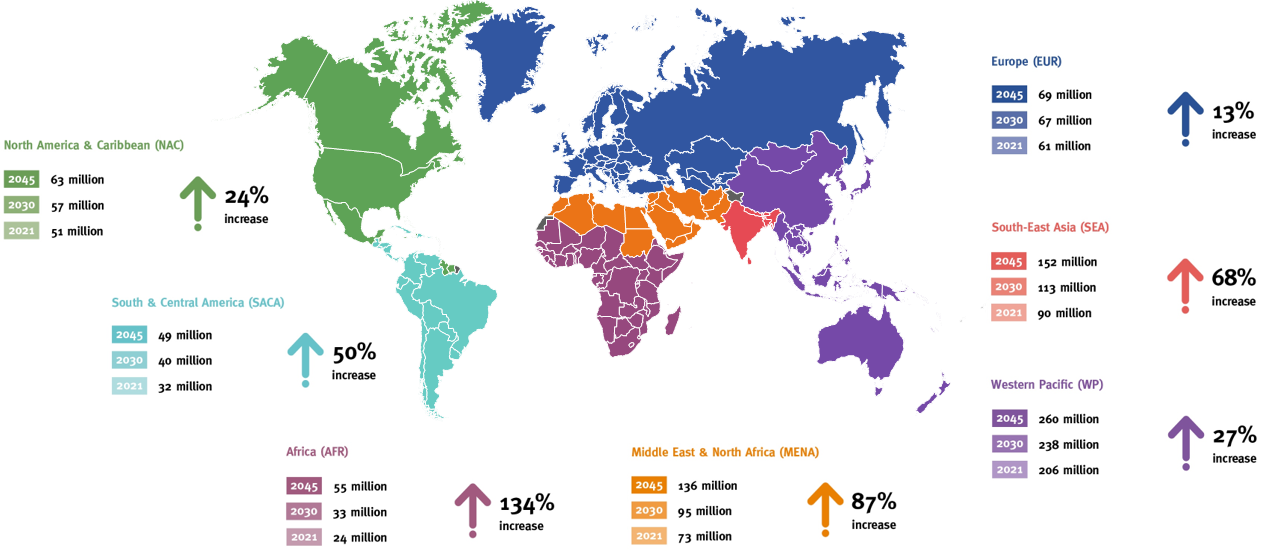
\includegraphics[width=15cm]{Chapter1/Fig/F1-3-01.png}
\caption[]{\textbf{IDF Atlas 2021}.\\
Percentages of diabetes cases around the world and projected increases by 2045}
\label{fig:idf}
\end{figure}


Consequently, diabetes stands as one of the foremost causes of global mortality \st{Altogether, this makes diabetes a leading cause of mortality worldwide} with 6.7 million deaths in 2021 \textbf{\cite{home_idf_nodate}}. These premature deaths and comorbidities \st{due to diabetes} inflict a huge economic strain on healthcare systems. The IDF estimated an expenditure of at least USD 966 billion in diabetes related causes in 2021 \textbf{\cite{home_idf_nodate}}. To address this burgeoning crisis and mitigate risk factors a multifaceted approach is essential with research efforts directed towards unraveling the complex interplay of genetic, environmental, and lifestyle factors that contribute to the development of diabetes. 



% ********************************** % 1.3.1  **************************************
\subsection{Forms of Diabetes} %Section - 1.3.1 
\label{sec:forsmDiabets}

DM \st{Diabetes mellitus (short - diabetes)} is \st{a group of complex metabolic disorders} characterized by sustained high blood glucose concentrations (hyperglycemia) \st{because of insufficient supply of insulin} resulting from inadequate insulin production, impaired insulin action, or a combination of both. Diabetes is broadly classified into two main types: Type 1 and Type 2  The current classification relies both disease etiology and pathogenesis \textbf{\cite{banday_pathophysiology_2020}}, serving as a valuable tool in clinical disease assessment and therapy determination. Based on this, diabetes can be divided into four main categories:\\
\begin{enumerate}
    \item Type 1 DM \textbf{(T1DM)}
    \item Type 2 DM \textbf{(T2DM)} 
    \item Gestational DM \textbf{(GDM)} and 
    \item Diabetes associated with certain specific conditions and/or disorders.
\end{enumerate}


%\begin{figure}[htbp]


\subsection{Type-1 Diabetes Mellitus (T1DM)}

Type-1 DM (T1DM) is a chronic, autoimmune disorder in which the insulin-secreting \textbeta-cells are progressively lost, and immune cell infiltration into the pancreatic islets play a crucial role in this process. The destruction of \textbeta-cells, caused by auto-reactive CD4 and CD8 T-cells results in little to no insulin production causing hyperglycaemia. As the disease progresses, auto-antibodies targeting \textbeta-cell proteins, especially native insulin, manifest and are subsequently joined by auto-antibodies against other proteins (glutamic acid decarboxylase or zinc transporter 8), leading to an expansion of auto-reactivity and eventual development of overt clinical disease (marked by destruction of 85-90\% of \textbeta-cells).
\newpage
T1DM is typically \st{presents during} diagnosed in childhood and adolescence,\st{but not exclusively, and accounts for 5-10\% of all cases of diabetes} although it can occur at any age, contributing to 5-10\% of all diabetes cases \textbf{\cite{banday_pathophysiology_2020}}. The etiology of T1DM is multifactorial, involving both, genetic predisposition and environmental triggers \st{play an important role in in its the pathogenesis. of T1DM}. The current therapeutic strategy entails daily exogenous administration of insulin to maintain stable glucose levels. Alternative approaches include a hybrid-closed loop model (artificial pancreas) for regulated insulin delivery, primary islet transplantation or immuno-modulation, albeit, the latter two present their own set of challenges. Additionally, early clinical trials involving stem cell therapies, such as mesenchymal stem cell (MSC) therapy have shown promising results as potential treatments for T1DM \textbf{\cite{pathak_therapies_2019}}.

\begin{figure}[t]
\centering
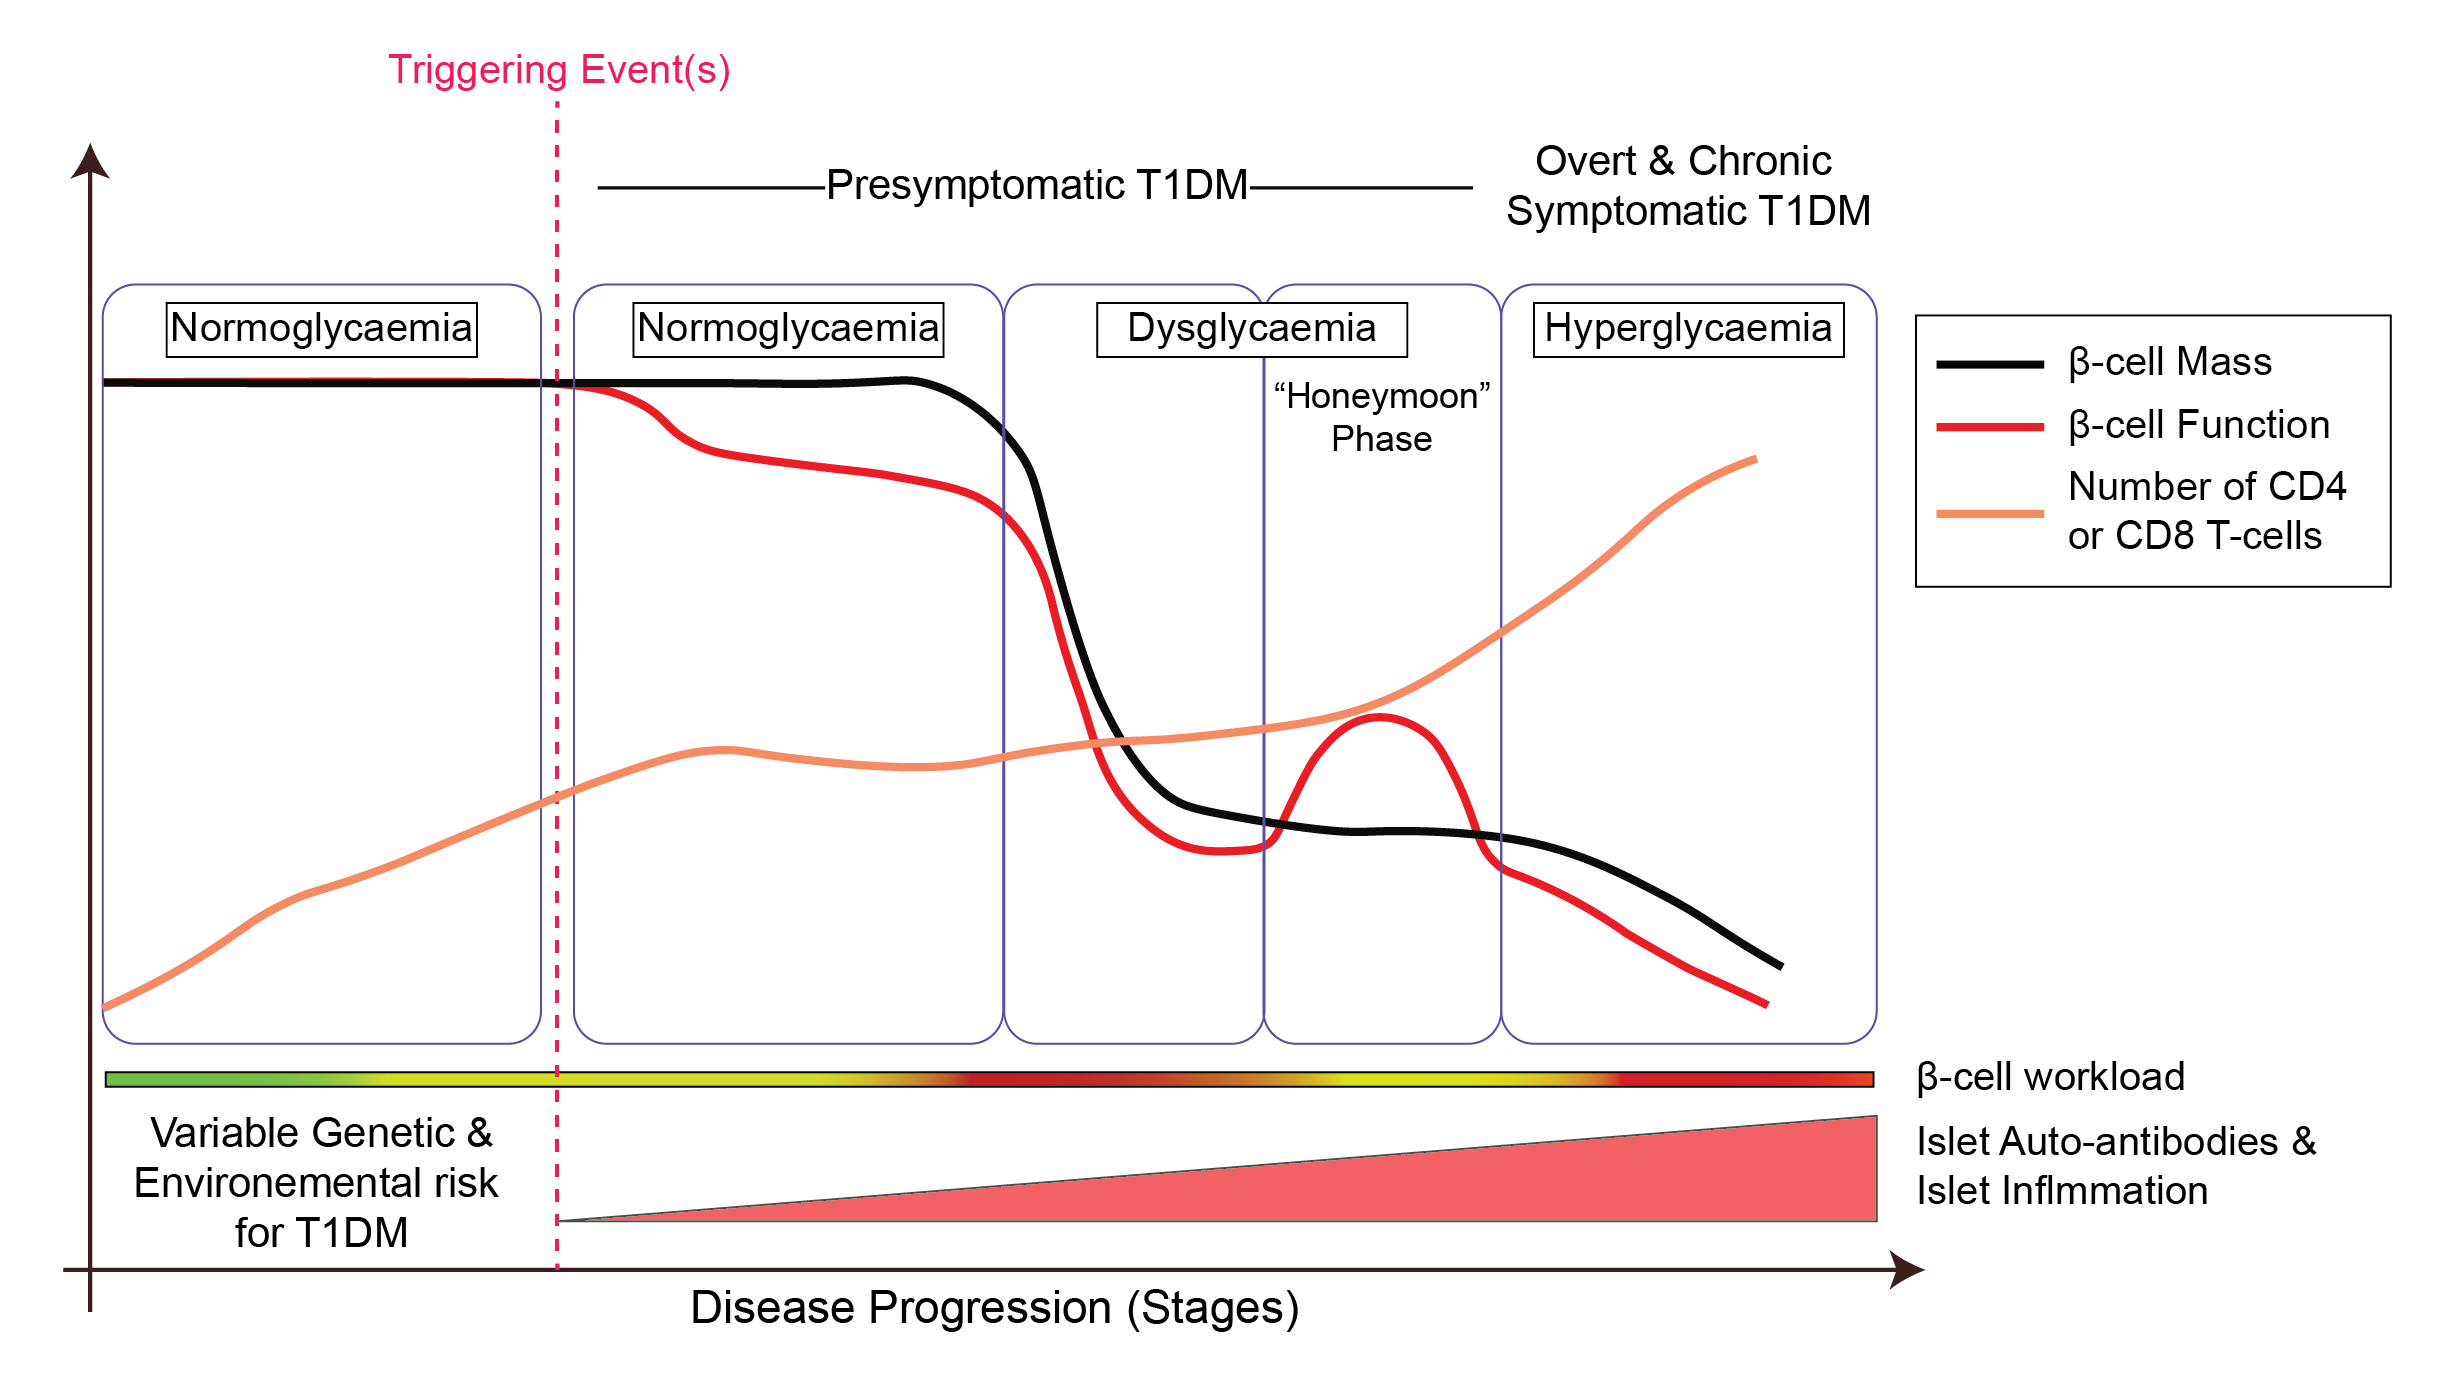
\includegraphics[width=16cm]{Chapter1/Fig/F1-3-02.png}
\caption[diabetes]{\textbf{T1DM pathogenesis}.\\
Adapted from several manuscripts that still need to be referenced here \textbf{\cite{chen_human_2017,von_herrath_type_2007,powers_type_2021}}}
%\label{fig:ipsc}
\end{figure}


\subsection{Type-2 Diabetes Mellitus (T2DM)}

Type-2 DM (T2DM) develops from high insulin demand due to insulin resistance in peripheral target tissues. The insulin resistant state manifests several years prior to T2DM diagnosis. Functional β-cells can match the increased metabolic demand by secreting more insulin in order to maintain normal glucose levels. However, sustained demand over chronic periods leads to progressive β-cell dysfunction, resulting in glucose intolerance and overt disease. \textbf{Insulin resistance and β-cell dysfunction are considered as major hallmarks of T2DM \cite{banday_pathophysiology_2020}}. 
\\\\
While, genome-wide association studies (GWAS) have been able to identify the genetic susceptibility to T2D \textbf{\cite{grarup_genetic_2014, wang_genetic_2016}}, other factors, particularly obesity have demonstrated a strong link to insulin resistance and T2DM pathogenesis. Excessive obesity causes a metabolic overload of the adipose tissue, resulting in chronic inflammation via secretion of pro-inflammatory cytokines such as TNF-a, IL-6, IL-1B and MCP-1 \textbf{\cite{guilherme_adipocyte_2008}}. The macrophages recruited into the adipose tissue create a chronically inflamed state and reduce the uptake of fatty acids by skeletal muscle. The elevated levels of these free fatty acids impair signaling and insulin-stimulated glucose transport leading to the development of insulin resistance \textbf{\cite{unger_lipotoxicity_1995,uysal_protection_1997,kanda_mcp-1_2006}}. However, the critical determinant for T2D is β-cell dysfunction \textbf{\cite{tahrani_glycaemic_2010, khin_pancreatic_2023}}, which is more severe than insulin resistance. The interplay between β-cell dysfunction and insulin resistance is highly complex; however, they likely influence each other and synergistically worsen T2DM.  Several factors are thought to contribute to β-cell dysfunction – chronic nutrient overload (glucotoxicity and glucolipotoxicity) \textbf{\cite{prentki_nutrient-induced_2020}}, insulin secretory defects \textbf{\cite{kahn_mechanisms_2006}}, reduced β-cell mass, amyloid deposition \textbf{\cite{prentki_islet_2006}} and/or islet inflammation and oxidative stresses. \st{The role of islet inflammation in T2D and its involvement in β-cell dysfunction is discussed at length in Chapter 2.}
\\\\
T2DM accounts for 90-95\% of all diagnosed diabetic cases \textbf{\cite{home_idf_nodate,banday_pathophysiology_2020,elsayed_2_2022}}. Due to the multi-faceted and progressive nature, the treatment for T2D follows a step-wise approach. The very first recommended therapeutic intervention is the adoption of a healthier life style: more healthy diet, increased physical activity and maintaining a healthy body weight. The first anti-diabetic drug to be usually prescribed is Metformin, which works by reducing hepatic gluconeogenesis, delaying intestinal absorption and improving the overall insulin sensitivity \textbf{\cite{kaneto_multifaceted_2021}}, although accumulating evidence points to possible new mechanisms of actions \textbf{\cite{foretz_metformin_2023}}. The persistence of T2DM further requires a additional medications as monotherapy is insufficient to maintain normal blood glucose levels \textbf{\cite{home_idf_nodate,nathan_medical_2009}}. Other available anti-diabetic drugs include sulphonylureas, GLP-1 agonists, thiazolidinediones, sodium-glucose cotransporter 2 (SGLT2) inhibitors or dipeptidyl peptidase 4 (DPP-4) inhibitors \textbf{\cite{home_idf_nodate,nathan_medical_2009,american_diabetes_association_8_2017}}. Upon failure of these antidiabetic drugs, intensive insulin therapy via exogenous administration becomes necessary in order to maintain the target range of blood glucose levels in T2DM patients and avoid health complications \textbf{\cite{home_idf_nodate}}.
\\\\

\subsection{Other forms of Diabetes}
T1DM and T2DM together account for most of the diabetes cases. Besides these two, there are also less common forms of diabetes:

\subsubsection{Gestational Diabetes Mellitus (GDM)}
Gestational diabetes mellitus (GDM) pertains to \st{is} any degree of glucose intolerance or diabetes diagnosed either at the onset of pregnancy or during its course \st{pregnancy}, usually in second or third trimester. Unlike preexisting diabetes in women, GDM usually resolves \st{soon after childbirth} shortly after childbirth or upon termination of pregnancy. \st{and is different from any preexisting diabetes in women.} Blood glucose levels undergo elevation during the third trimester, and when they reach diabetic levels, the condition is described as GDM. The risk of GDM increases with age, obesity, previous pregnancies and any previous history of glucose intolerance or GDM itself. Additionally, GDM has been associated with an increase lifetime risk of developing T2DM. Therefore, individuals need to be assessed for persistent diabetes postpartum, in order to ensure early diagnosis \textbf{\cite{banday_pathophysiology_2020,egan_what_2019}}.

\subsubsection{Latent Autoimmune Diabetes in Adults (LADA)}
Latent autoimmune diabetes in adults (LADA), also referred as Type-1.5 diabetes, exhibits clinical features similar to both T1DM and T2DM. It is the most common form of adult-onset autoimmune diabetes, accounting for 2-12\% of all diabetic cases. LADA is characterized by the presence of certain autoantibodies and its strong association with the human leukocyte antigen (HLA) region that are associated with immune response, including autoimmunity. Patients with LADA often exhibit insulin resistance similar to T2D. However, LADA is genetically distinct from both T1DM and T2DM despite sharing genetic risk factors \textbf{\cite{banday_pathophysiology_2020,carlsson_etiology_2019,andersen_latent_2010,andersen_type_2014,cervin_genetic_2008}}. 

\subsubsection{Monogenic Diabetes}
Monogenic diabetes arise \st{from defects in single gene}due to single-gene defects in contrast to the multifactorial etiologies of T1DM or T2DM\st{, which involved contributions of multiple genes and environmental factors}. Monogenic diabetes are less common contributing to 1.5 – 2\% of total diabetes cases, and are often misdiagnosed as either T1DM or T2DM. In recent years, with several genome-wide association studies, an increasing number of monogenic diabetes are being discovered\st{. Therefore, the true prevalence of this type may be underestimated.}, suggesting that its true prevalence might be underestimated. The spectrum of  monogenic diabetes encompasses conditions such as \st{forms present a broad spectrum from }maturity-onset diabetes of the young (MODY), neonatal diabetes mellitus (NDM) and rare diabetes-associated syndromic diseases \textbf{\cite{home_idf_nodate}}. 

\subsubsection{Maturity-onset diabetes of the young (MODY)}
Maturity-onset diabetes of the young (MODY)\st{, also known as monogenic diabetes,} results from mutations in several specific genes involved in pancreatic β-cell function thereby affecting glucose sensing and subsequent insulin secretion, with minimal to no defects in insulin action. As the name suggests, MODY demonstrates an early onset, with glucose intolerance and hyperglycemia manifesting usually before the age of 25, although it can occur late in life. It is distinct from both T1DM and T2DM and follows an autosomal dominant inheritance pattern. At least 14 genes associated with MODY have been identified so far and these are mostly located on different chromosomes. The most prevalent forms of MODY are designated as MODY2 (glucokinase gene, \textit{GCK}), MODY3 (transcription factor, \textit{HNF1A}) and MODY1 (transcription factor \textit{HNF4A}), together accounting for more than 80\% of MODY cases \textbf{\cite{banday_pathophysiology_2020,american_diabetes_association_2_2020}}.

\subsubsection{Neonatal Diabetes Mellitus (NDM)}
Neonatal diabetes mellitus (NDM) is a monogenic diabetes diagnosed during the \st{first 6} initial six months of life. The genetic abnormalities associated with NDM result in β-cell dysfunction and decreased β-cell mass due to increased apoptotic or non-apoptotic cell death leading to severe hyperglycemia along with hypoinsulinemia \textbf{\cite{banday_pathophysiology_2020}}. NDM is a rare disorder (incidence rate - 1 per 500,000 – 300,000 live births) \textbf{\cite{banday_pathophysiology_2020,iafusco_minimal_2012,polak_neonatal_2007}}  and is highly distinct from T1DM in both its origin and nature of inborn pancreatic disorder. The genetic defects also result in developmental \st{abnormalities}irregularities of pancreas and/or its islets and in extremely rare \st{cases} instances, their complete absence, leading to decreased insulin production and secretion, and in the latter case, an absolute deficiency, thereby requiring insulin replacement therapy. Based on the clinical presentation, NDM can be either transient (most common form – resulting from overexpression of genes on chromosome region \textit{6q24}) or permanent (less common form – resulting from heterozygous autosomal dominant mutations in the genes encoding for subunits of β-cell K\textsubscript{ATP channel}).%\clearpage
\\\\Furthermore, various other forms of diabetes arise from diverse contributing factors, which are elucidated in this comprehensive review \textbf{\cite{banday_pathophysiology_2020}}.
\\\\
In summary, DM is a complex and heterogeneous metabolic disorder characterized by persistent hyperglycaemia and loss of functional β-cell mass. The pathogenesis of DM involves several factors, including genetics and strong environmental influences. While there are effective and personalized treatments available for DM, these strategies do not halt the progression of the disorder. Therefore, management of DM involves lifelong medication and continuous care to maintain health and prevent secondary complications. 
%The overall aim of this thesis is to provide suitable computational methods for the identification of cell type and context-specific eQTL using single cell expression profiles, and explore their application across a range of human iPSC-derived cell types, using data from the \gls{hipsci} project.\\

%Specifically, in \textbf{Chapter \ref{chapter2}}, I provide an overview of the use of linear and \glspl{lmm} for genetic association analyses, focusing on their application in \gls{eqtl} mapping.\\

%In \textbf{Chapter \ref{chapter3}}, I describe best-practice approaches to perform \gls{eqtl} mapping using \gls{scrnaseq} profiles and demonstrate these methods on matched bulk and single cell expression of around 100 human \gls{ipsc} lines. \\

%In \textbf{Chapter \ref{chapter4}}, I present a dataset of almost 40,000 cells from 125 human \gls{ipsc} lines differentiating to definitive endoderm, and demonstrate different approaches to \gls{eqtl} mapping using \gls{scrnaseq} data, identifying genetic variants that affect gene expression dynamically along differentiation and across other cellular states. \\

%In \textbf{Chapter \ref{chapter5}}, I present a dataset of over one million cells from 215 human \gls{ipsc} lines differentiating to midbrain dopaminergic neurons. We identify thousands of \glspl{eqtl} across a number of cell types and upon external stimulation. In addition, we identify hundreds of colocalisation events with variants that are known to be associated with neurological traits and diseases. Moreover, we investigate sources of variation in the capacity of individual cell lines to differentiate toward neurons.\\

%Finally, in \textbf{Chapter \ref{chapter6}}, I conclude and discuss future directions.
\newpage

% ***************************************************************
%************************ %Fourth Section %****************************************************************
\section{scRNA-seq}  %Section - 1.4
\label{sec:scrna} 

\subsection{Introduction}
\label{sec:141}


\subsection{Other Modalities}
\label{sec:142}

Besides single-cell transcriptomics, a range of other technologies aims to profile the distinct layers contributing to the overall molecular make-up of a cell. Collectively, these single-cell methodologies enable us to uncover cellular diversity from novel perspectives, offering comprehensive and impartial analyses of individual cells \textbf{\cite{stein_single-cell_2021}}. Some of these modalities are:

\subsubsection{Single-cell multi-omics}

As discussed in the previous sections, the various single-cell ‘single-omics’ methods have generated a vast array of data from individual modalities, thereby allowing the examination of cellular properties and the dissection of the mechanisms of gene regulation at a single-cell level. While these single modalities provide important insights, the combination of data across these modalities results in much finer insights about individual cells and provides information about the interaction between the various layers for any given cell-type or cell-state. In addition, multi-modal analyses can provide complementary information between layers due to the inherent differences between them and improve our ability to identify cell-types and cell-states \textbf{\cite{flynn_single-cell_2023}}. \st{Multi-omics analyses has been applied on tumours at a bulk level and provided a comprehensive understanding of cellular processes through integration of data on mutations, mRNA, proteins and metabolites} \textbf{\cite{lee_single-cell_2020}}.
\\\\
This has prompted the development of single-cell multi-omics technologies which allow for simultaneous profiling of genome, epigenome, transcriptome, proteome and other modalities. Further, single-cell multi-omics technologies have seen continuous improvements in multiplexing, throughput, resolution and accuracy. Several multi-omics methods utilize the transcriptome profiling as an ‘anchor’ to facilitate downstream integration of the several layers \textbf{\cite{baysoy_technological_2023}}. The transcriptome profiling can be combined with genomics (G\&T-seq \textbf{\cite{macaulay_gt-seq_2015}}), epigenome (scM\&T-seq \textbf{\cite{angermueller_parallel_2016}}, scNMT-seq \textbf{\cite{clark_scnmt-seq_2018}}), proteomics (CITE-seq \textbf{\cite{stoeckius_simultaneous_2017}}) or other modalities \textbf{\cite{dixit_perturb-seq_2016,singh_high-throughput_2019}}, offering a multi-layered approach to single-cell analysis. Alongside the development of these technologies, computational strategies to deal with the challenges of combining diverse datasets from various omics layers have also advanced significantly, with current methods employing regression or association techniques, unsupervised integration, data-ensemble, model-ensemble \textbf{\cite{vahabi_unsupervised_2022, stanojevic_computational_2022}} or deep-learning algorithms \textbf{\cite{baysoy_technological_2023,athaya_multimodal_2023}}. The complexity and high-dimensionality of single-cell multi-omics data presents several challenges for computational approaches such as a lack of harmonized data format across modalities, the non-alignment of modalities in case of unpaired datasets, the multiplication of technical noise across several layers, all of which require continuous development and refinement of these methods.
\\\\
In summary, single-cell multi-omics technologies offer immense potential in elucidating complex biological processes in health and diseases by simultaneously capturing complementary information from various biological layers. These techniques and their corresponding computational methods require improvement and benchmarking in order to enhance their accuracy, scalability, and usability, ultimately empowering researchers to gain deeper insights into cellular heterogeneity, regulatory networks, and disease mechanisms. For further reading, interested readers can refer to several reviews summarizing the various technologies and their applications, computational tools to analyze multi-modal data as well as discussions on current challengers and future perspectives in this field \textbf{\cite{flynn_single-cell_2023,lee_single-cell_2020,baysoy_technological_2023, miao_multi-omics_2021, dimitriu_single-cell_2022}}. 
\clearpage
\subsection{Single-cell \textit{-omics} in pancreas}
\label{sec:143}
The rapid growth and development of single-cell transcriptomics and other \textit{–omics} assays have greatly advanced our understanding of pancreatic physiology, including development, cellular heterogeneity (including rare cell-types) and disease mechanisms. For a greater overview of findings from multiple studies in this space, the readers can refer here \textbf{\cite{wang_single-cell_2019,avrahami_beta_2017,carrano_interrogating_2017}}. A major outcome from the application of scRNA-seq is the refinement of cell-type specific gene signatures, including the identification of rare ghrelin-producing ε cells in the human pancreas \textbf{\cite{segerstolpe_single-cell_2016}}. Several scRNA-seq studies have identified heterogeneity of beta-cells within islets, with subtypes \textbf{\cite{segerstolpe_single-cell_2016}} or cell states exhibiting differential markers for endoplasmic reticulum (ER) stress \textbf{\cite{baron_single-cell_2016,muraro_single-cell_2016}} and oxidative response \textbf{\cite{muraro_single-cell_2016}} as well as groups with expression of maturation markers.\\\\
In recent years, researchers have utilized scRNA-seq to investigate both endocrine and exocrine pancreatic lineages, developmental trajectories and regulatory mechanisms of intermediate progenitor populations along the developmental pathway. One such study identified multiple stages of endocrine precursor cell differentiation before the allocation of islet lineage in several reporter mouse strains \textbf{\cite{yu_defining_2019}}. In a more recent single-cell spatio-temporal study, the authors depicted that the islet morphology and endocrine differentiation are closely related and that the islets form as budding ‘peninsulas’ as opposed to aggregation of dispersed cells \textbf{\cite{sharon_peninsular_2019}}. In this peninsular morphology, α-cells develop first in the outer layer and β-cells develop later, beneath them, thereby reflecting eventual mature islet architecture. Another study involving human fetal pancreas in second trimester identified an uncommitted multipotent progenitor cells directing self-renewal and pancreatic organogenesis \textbf{\cite{villani_sox9ptf1a_2019}}.\\\\ 
By mapping individual β-cells from mouse pancreata along an ‘inferred’ maturation trajectory, two studies identified signatures of immature β-cells \textbf{\cite{qiu_deciphering_2017,zeng_pseudotemporal_2017}}. The pseudotemporal analysis of postpartum β-cell development depicted a crucial role for ROS and amino acids, with the algorithm proclaiming significant changes in β-cell metabolism during early postnatal period. A similar analysis of β-cells from human non-diabetic deceased donors suggested that β-cells are separated by states of high insulin biosynthesis followed by recovery from the ensuing ER stress by activation of unfolded protein response (UPR) pathway \textbf{\cite{xin_pseudotime_2018}}.  Interestingly, the algorithm revealed a branching pattern among the β-cell states indicating potential β-cell subpopulations, similar to previous studies.\\\\
As discussed in the earlier section, the two major types of diabetes are associated with autoimmune destruction (T1DM) of β-cells or with the dysfunction and loss (T2DM) of β-cells, leading to insulin resistance. Therefore, a major goal of diabetes research is the replenishment of missing or abnormal β-cells. A single-cell mRNA and CRISPR screen study identified several genes at obesity loci and T2DM loci associated with β-cells. Obesity is a major risk factor in the development of T2DM and the study identified various genetic commonalities between the two diseases \textbf{\cite{fang_single-cell_2019}}. In another study, the authors utilized snATAC-seq assay to uncover heterogeneity in regulatory programs of β-cell states and that the genetic risk of T2D is likely mediated through a state of high insulin production and other functional states related to stress and signaling responses \textbf{\cite{chiou_single-cell_2021}}. Moreover, the study also implicated other endocrine cell types, particularly δ-cells, with the genetic risk of T2DM. A comparative study of three single-cell transcriptomic datasets of T2DM donors using machine-learning classifiers found that in T2DM, β-cells normally express insulin under low cellular stress and exhibit abnormal functionality upon high stress conditions \textbf{\cite{ma_single-cell_2018}}. In addition, correlation analysis depicted that oxidative stress could represent a crucial factor in influencing insulin expression in T2DM patients and that expression is also individual-specific. 
\\\\
<NEED 1 more PARAGRAPH TO ROUND OUT THE SECTION>

\clearpage
\subsection{Data analysis methods}
\label{sec:144}

\subsubsection{Ambient mRNA contamination}
During library preparation in droplet-based single-cell technologies, cells that are stressed or undergoing apoptosis, may release their mRNA content into the cell suspension. These freely floating transcripts in the background are referred to as \textbf{‘ambient mRNA’} and can cross-contaminate the endogenous gene expression profiles of cells, thereby complicating downstream analysis steps, such as cell-type annotation \textbf{\cite{yang_decontamination_2020}}. Apart from this, high background mRNA counts could also occur when working with specific tissues \textbf{\cite{10x_genomics_introduction_nodate,madissoon_scrna-seq_2019}}; while employing nuclei isolation protocols which typically release cytoplasmic RNA into the solution \textbf{\cite{10x_genomics_introduction_nodate}}; from abundant cell-types whose RNA can contaminate the less abundant cell-types \textbf{\cite{10x_genomics_introduction_nodate,caglayan_neuronal_2022}} or from other exogeneous sources of contamination \textbf{\cite{10x_genomics_introduction_nodate}}. Therefore, accounting for background RNA profiles in scRNA-seq data is necessary to ensure the reliability and accuracy of results of downstream data analysis. Several computational tools have been developed to identify and remove ambient mRNA \textbf{\cite{yang_decontamination_2020,young_soupx_2020,fleming_unsupervised_2023,yan_emptynn_2021,alvarez_enhancing_2020,muskovic_dropletqc_2021}}. These tools work to either remove entire droplets based on their corresponding expression profiles or remove the ambient mRNA associated with barcodes.\footnote{Ultimately, the use of background correction tools depend on the extent of the contamination as well as the overall goals of the experiment. It is recommended to carefully inspect the data beforehand as not every dataset might require ambient mRNA correction.\\}
\vspace{3mm}
\begin{Abstract}
\vspace{3mm}
The following section provides a descriptive explanation of SoupX \textbf{\cite{young_soupx_2020}}, which is one of the several aforementioned computational tools for the estimation and correction of ambient mRNA. In \textbf{Chapter 2} and \textbf{Chapter 3}, I have used SoupX as part of the pre-processing workflow in order to account for background contamination. 
\vspace{3mm}
\end{Abstract}
\vspace{3mm}
SoupX is a computational method that quantifies the extent of ambient mRNA contamination and recovers true, cell-specific signal. The authors refer to the input solution with the floating cell free mRNAs as \textbf{‘the soup’}. The method consists of three steps:
\begin{enumerate}
    \item Estimate the composition of the soup.
    \item Compute the \st{cell-specific} contamination fraction ($\mathbf{\rho}$) and
    \item Generate a corrected count matrix after removing the soup-based expression.
\end{enumerate}
SoupX estimates the profile the the soup from the empty droplets in the scRNA-seq data. In an 10x Chromium experiment, this corresponds to the \textbf{‘unfiltered feature-barcode’} matrix file. The expression profile of the soup is automatically estimated from the empty droplets and the counts data. In cases, when the empty droplets file might be unavailable, the profile of the soup can be estimated manually. An important intermediate step is to provide the clustering information for each sample which renders the subsequent correction step more robust. Next, the level of background contamination ($\mathbf{\rho}$) in each sample is estimated and can be accomplished in two ways: \textbf{the automatic method to estimate the contamination fraction} or \textbf{the manual method, by providing a list of ‘non-expressed’ genes}. Skipping these methods, the contamination fraction can also be set directly at a fixed value.\footnote{As SoupX is designed to be conservative, manually setting a global contamination fraction can remove a greater proportion of the background with a low risk of losing true biological signals.}
\newpage
For the automatic estimation, SoupX makes use of highly-expressed cluster-specific markers to estimate $\mathbf{\rho}$ for every gene, against the clusters in which it can be confidently said to not be expressed. Using the estimates of these gene-cluster pairs, SoupX calculates a posterior distribution, using a Poisson-likelihood, of the contamination fraction and determines its best estimate. Therefore, to get a better estimate of $\mathbf{\rho}$, it is imperative to have, for every set of cells, a list of genes that is known to not be expressed in that set and by measuring the expression of those genes, the global contamination fraction can be estimated. 


\subsubsection{Cell-Cell Interactions}
Cells, that make up the tissues, constantly coordinate with each other and their microenvironment. This allows cells to maintain homeostasis, respond to internal and external perturbations, thereby allowing the tissue to function properly. In the absence of proper interactions and coordination, disease ensues. This complex coordination is a result of \textbf{cell-cell interactions (CCIs)} \textbf{\cite{armingol_deciphering_2021}} whereby cells can send or received biochemical and physical signals, that ultimately influence phenotype and function. Cells can interact and influence via specific signalling molecules such as ligands (growth factors, chemokines, cytokines), receptors, metabolites, ions, and structural or secreted proteins from the extracellular matrix \textbf{\cite{armingol_deciphering_2021,armingol_diversification_2024}}. In particular, interactions mediated through ligands from sender cells and the corresponding cognate receptors on receiver cells are also known as \textbf{cell-cell communication (CCC)}, which culminates in altered gene expression \textbf{\cite{armingol_deciphering_2021,armingol_diversification_2024}}. Therefore, it is crucial to understand how cells interact and communicate, in order to shed light on potential mechanisms underlying biological processes such as development and disease progression. The combination of single-cell transcriptomics and high-confidence \textbf{ligand-receptor interaction (LRI)} databases, has made it possible to infer putative intercellular communications by examining the co-expression of genes corresponding to the ligand-receptor pairs \textbf{\cite{wilk_comparative_2023}}. A plethora of computational tools have been developed to infer CCIs from transcriptomics data. These tools have been reviewed in-depth and extensively bench-marked, and I direct the readers to these publications for further reading \textbf{\cite{armingol_deciphering_2021,armingol_diversification_2024,liu_evaluation_2022,xie_comparison_2023,cheng_review_2023}}
\vspace{3mm}
\begin{Abstract}
\vspace{3mm}
In the following section, I will briefly describe and summarize CellChat \textbf{\cite{jin_inference_2021}}, a computational tool, designed to infer CCIs from scRNA-seq data. CellChat is considered as a ‘core’ tool	which established a set of methods and is widely used by the scRNA-seq community \textbf{\cite{armingol_diversification_2024}}.
\vspace{3mm}
\end{Abstract}
\vspace{3mm}
To infer CCIs from scRNA-seq data, CellChat makes use of \textbf{CellChatDB}, a database of literature supported LRIs, in both mouse and human. CellChatDB is specific as it contains LRIs involving multimeric receptors, cofactor molecules as well as co-stimulatory or co-inhibitory membrane bound receptors, and is grouped into several signalling pathway families. In addition, CellChatDB allows for updating of the database by adding user-defined ligand-receptor pairs. Next, to infer intercellular communications from scRNA-seq data, CellChat first identifies differential signalling genes across all cell-types in the data using the Wilcoxon rank sum test, and for these differential genes, computes the \textbf{“ensemble average expression”} in the cell-type. Following this, a communication probability value for every LRI pair is modelled based on the \textbf{Law of Mass Action} and a \textbf{Hill function}. By using the expression levels of ligands and receptors as “proxies” for their concentration and modelling interactions with expression-based Hill functions \footnote{In CellChat, the Hill function is used to incorporate the effects of positive and negative effectors into the framework, thereby providing a more nuanced and accurate model of cell-cell communication}. In addition, the frequencies of the cell-types are also accounted for in the probability calculation. Finally, significant interactions between two cell-types are identified on the basis of a random permutation test <add footnote here>   . Using centrality metrics from graph theory, CellChat identifies higher order information from a weighted-directed network, wherein the computed communication probabilities are used as weights. This allows for the identification of dominant signalling sources as well as mediators and influencers within the network. CellChat can also predict key outgoing and incoming signals for specific cell-types as well as coordinated responses amongst different cell-types by pattern recognition approaches based on non-negative matrix factorization. An important application of CellChat is the joint analyses of two or more datasets by constructing a shared manifold space using a shared nearest neighbour (SNN) similarity network. This enables the identification of conserved as well as context-specific interactions between the datasets being compared.    